\chapter{Implementación}

    \section{Aritmética de punto fijo}
        
        Cuando se necesita trabajar con números de punto decimal en dispositivos digitales se puede optar por utilizar aritmética de punto fijo o aritmética de punto flotante. La aritmética de punto fijo en comparación de la de punto flotante tiene la ventaja de ser más rápida y utilizar menos recursos, sin embargo, tiene la desventaja de tener un rango de uso específico el cual se tienen que establecer al principio del diseño y el cual no puede modificarse posteriormente. Por el contrario la aritmética de punto flotante tienen un mayor rango dinámico y resulta útil cuando los algoritmos tienen una complejidad alta. 

        En el proceso de diseño de arquitecturas digitales de aplicación especifica se busca utilizar la menor cantidad de recursos y reducir al máximo el tiempo de ejecución del algoritmo subyacente. Cuando se trabaja con los FPGA se cuenta con la libertad de poder analizar y estudiar el algoritmo antes de comenzar con el proceso de diseño. Por todo lo anterior, es preferible utiliza operaciones en punto fijo en lugar de punto flotante en los FPGA \cite{TleloCuautle2016}.

        La representación de punto fijo de un número $X$ es $X(a,b)$ donde $a$ es la parte entera y $b$ es la parte fraccionario. De manera que el número de bits de la representación es $a+b+1$, es decir las suma de la parte entera, la parte fraccionaria y el bit de signo. El rango de valores que se puede representar es $[-2^{a}, 2^{a} - 2^{-b}]$ y por lo tanto el número más pequeño que puede representar o visto de otro modo la precisión es de $2^{-b}$. En la Tabla \ref{tab:ejemplos_puntofijo} se muestran ejemplos de diferentes formas de interpretar números binarios  utilizando 5 bits y diferentes formatos de punto fijo.
        
        Cuando se hace la suma de dos números de punto fijo $X(a,b)$, ambos números tienen un rango de $[-2^{a}, 2^{a} - 2^{-b}]$. El mayor número que se puede obtener sumando dos extremos, los dos más positivos o los dos más negativos. Sumando los dos más negativos se obtiene:

        \begin{equation}
            -2^{a} + (-2^{a}) = 2 (-2^{a}) = -2^{a+1}
            \label{eq:}
        \end{equation}
        sumando los dos más positivos:

        \begin{equation}
            (2^{a} - 2^{-b}) + (2^{a} - 2^{-b}) = 2 (2^{a} - 2^{-b}) = 2^{a+1} - 2^{1-b}            
            \label{eq:}
        \end{equation}
        y como $|-2^{a+1}| > |2^{a+1} - 2^{1-b}|$. Entonces hay que representar el mayor número negativo número $-2^{a+1}$.

        Entonces el resultado de la suma de dos números de punto fijo $X(a,b)$ es un número $X(a+1,b)$. Por ejemplo, si sumamos dos números con el formato de punto fijo $X(3,0)$, el mayor número se genera sumando $-8-8 = -16$. Este resultado necesita una representación $X(4,0)$, que tiene un rango de $[-16,15]$.

        \begin{table}[htbp]
            \centering
            \caption{Ejemplos de formato, rango y conversión de números de 5 bits en formato de punto fijo.}
            \begin{tabular}{|l|l|l|l|}
                \hline
                \rowcolor{lightgray}   Número & Conversión & Formato $X(a,b)$  & Rango $[-2^{a}, 2^{a} - 2^{-b}]$\\
                01110 & 3.5 & $X(2,2)$ & $[-4,3.75]$ \\ 
                \hline
                10010 & -3.5 & $\cdots$ & $\cdots$\\ 
                \hline
                00011 & 0.75 & $\cdots$ & $\cdots$\\ 
                \hline
                01110 & 1.75 & $X(1,3)$ & $[-2,1.875]$ \\ 
                \hline
                10010 & -1.75 & $\cdots$ & $\cdots$\\ 
                \hline
                00011 & 0.375 & $\cdots$ & $\cdots$\\ 
                \hline
                01110 & 7.0 & $X(3,1)$ & $[-8,7.5]$ \\ 
                \hline
                10010 & -7.0 & $\cdots$ & $\cdots$\\ 
                \hline
                00011 & 1.5 & $\cdots$ & $\cdots$\\ 
                \hline
            \end{tabular}
            \label{tab:ejemplos_puntofijo}
        \end{table}

        Para una multiplicación de dos números $X(a,b)$, analizamos cuantos bits se requieren para almacenar el resultado. Los números más grandes que se generan son el resultado más positivo generado al multiplicar ambos números negativos, y el más negativo, resultado de multiplicar el más positivo y el más negativo. Para los dos más negativos tenemos:
        
        \begin{equation}
            (-2^{a})(-2^{a}) = 2^{2a}
        \end{equation}
        para el más positivo y el más negativo tenemos:
        
        \begin{equation}
            (-2^{a})(2^{a}-2^{-b}) = -2^{2a} + 2^{a-b}
        \end{equation}
        y a multiplicación de los dos más positivos es:

        \begin{equation}
            (2^{a} - 2^{-b}) = 2^{2a} - 2^{-2b}
        \end{equation}

        El número positivo más grande que es necesario representar es $2^{2a}$. También es necesario representar $-2^{-2b}$, entonces se necesita el número $X(2a+1,2b)$ para representar la multiplicación de dos números $X(a,b)$. $X(2a+1,2b)$ tiene un rango de $[-2^{a+1}, 2^{2a+1} - 2^{-2b}]$.

        
	\section{Mapa caótico}
    
        En el artículo \cite{Sprott1993} se analiza y estudia el mapa caótico cuadrático bidimensional más sencillo que esta dado por la ecuación (\ref{eq:mapa2d}). 
        \begin{equation}
            \begin{array}{ccl}
                x_{n+1} & = &  a_{1} + a_{2}x_{n} + a_{3}x_{n}^{2} + a_{4}x_{n}y_{n} + a_{5}y_{n} + a_{6}y_{n}^{2}\\
                y_{n+1} & = &  a_{7} + a_{8}x_{n} + a_{9}x_{n}^{2} + a_{10}x_{n}y_{n} + a_{11}y_{n} + a_{12}y_{n}^{2}
            \end{array}
            \label{eq:mapa2d}
        \end{equation}
        donde los parámetros $\{a_{1}, a_{2}, \ldots a_{12}\}$ y las condiciones iniciales $x_{0}$ y $y_{0}$ determinan las características de la solución. La iteraciones se representan como puntos en una superficie bidimensional. Después de un cierto número de iteraciones, la solución hará una de estas cuatro cosas: (a) convergerá a un único punto fijo; (b) tomará una sucesión de valores que acabarán repitiéndose, produciendo un ciclo límite; (c) será inestable y divergirá hasta el infinito; (d) mostrará caos y rellenará gradualmente alguna región a menudo complicada pero acotada del plano $x-y$.
        
        Para saber qué valores de $\{a_{1}, a_{2}, \ldots a_{12}\}$ llevan al caos, \cite{Sprott1993} utilizó el siguiente procedimiento.

        \begin{enumerate}
            \item Elegir aleatoriamente los 12 coeficientes de $a_{1}$ hasta $a_{12}$ aleatoriamente sobre algún intervalo.
            \item Elegir las condiciones iniciales $x_{0}$ y $y_{0}$.
            \item Iterar las ecuaciones del mapa mientras se calcula el exponente de Lyapunov y se comprueba si no hay divergencia.
            \item Mantener las soluciones que están acotadas y tienen un exponente de Lyapunov positivo.
        \end{enumerate}

        Los coeficientes los eligió en incrementos de 0.1 en el intervalo de $-1.2$ a $1.2$, es decir, 25 valores posibles. Coeficientes más pequeños hacen que se pierdan muchas soluciones caóticas y más grandes producen sobre todo soluciones inestables. El incremento se eligió para que cada atractor sea visiblemente diferente y los coeficientes puedan codificarse en letras del alfabeto desde la $A$ hasta la $Y$. De manera que $A = -1.2, B = -1.1, C = -1.0, \ldots, Y = 1.2$. La Tabla \ref{tab:conversion_mapas} puede utilizarse para realizar la conversión de esta representación de manera rápida. Esta representación hace que sea fácil su replicación. Así, cada atractor se identifica unívocamente con un nombre de 12 letras. El número de posibles casos es $25^{12}$ o aproximadamente $6\times 10^{12}$. De estos, aproximadamente 1.6\% son caóticos. Verlos todos a un ritmo de uno por segundo requeriría más de 30 millones de años. Por tanto, es muy poco probable que los patrones producidos se hayan visto antes y, al igual que los copos de nieve, casi todos son diferentes.

        \begin{table}[htbp]
            \centering
            \caption{Conversiones para codificación de los atractores.}
            \begin{tabular}{|l|l|l|l|}
                \hline
                \rowcolor{lightgray}   Letra & Codificación & Letra & Codificación\\
                A & -1.2 & N & 0.1 \\ 
                \hline
                B & -1.1 & O & 0.2 \\ 
                \hline
                C & -1.0 & P & 0.3 \\ 
                \hline
                D & -0.9 & Q & 0.4 \\ 
                \hline
                E & -0.8 & R & 0.5 \\ 
                \hline
                F & -0.7 & S & 0.6 \\ 
                \hline
                G & -0.6 & T & 0.7 \\ 
                \hline
                H & -0.5 & U & 0.8 \\ 
                \hline
                I & -0.4 & V & 0.9 \\ 
                \hline
                J & -0.3 & W & 1.0 \\ 
                \hline
                K & -0.2 & X & 1.1 \\ 
                \hline
                L & -0.1 & Y & 1.2 \\ 
                \hline
                M & -0.0 &   &     \\ 
                \hline
            \end{tabular}
            \label{tab:conversion_mapas}
        \end{table}

        Algunos de los atractores más llamativos se muestran en la Figura \ref{fig:multiples_atractores} y se pueden obtener decodificando la palabra de 12 letras de la Tabla \ref{tab:codificacion} del atractor deseado. En el artículo \cite{Sprott1993} no se tienen en cuenta las posibles variaciones que pueden ocurrir al modificar las condición iniciales. Estas se eligieron arbitrariamente a $x_{0} = y_{0} = 0.05$, además, no se especifica el rango que pueden tener las condiciones iniciales en el que se asegure que exista el caos.

        \begin{table}[htbp]
            \centering
            \caption{Diversos identificadores, dimensión fractal y exponente de Lyapunov para atractores del mapa caótico bidimensional.}
            \begin{tabular}{|l|l|l|l|}
                \hline
                \rowcolor{lightgray}  Atractor & Identificador & Dimensión fractal & Exponente de Lyapunov \\
                \hline
                1     & \verb|GLXOESFTTPSV| & 1.77  & 0.12   \\ %e
                \hline
                2     & \verb|CVQKGHQTPHTE| & 1.79  & 0.14   \\ %b
                \hline
                3     & \verb|UWACXDQIGKHF| & 1.42  & 0.10   \\ %n
    \hline
                4    &  \verb|GIIETPIQRRUL| & 1.50  & 0.13   \\ %d
                \hline
                5     & \verb|MCRBIPOPHTBN| & 1.39  & 0.05   \\ %j
                \hline
                6     & \verb|ODGQCNXODNYA| & 1.31  & 0.07   \\ %l
                \hline
            \end{tabular}
            \label{tab:codificacion}
        \end{table}

        \begin{figure}[hbtp]
            \centering
            \begin{subfigure}[b]{0.475\textwidth}
                \centering
                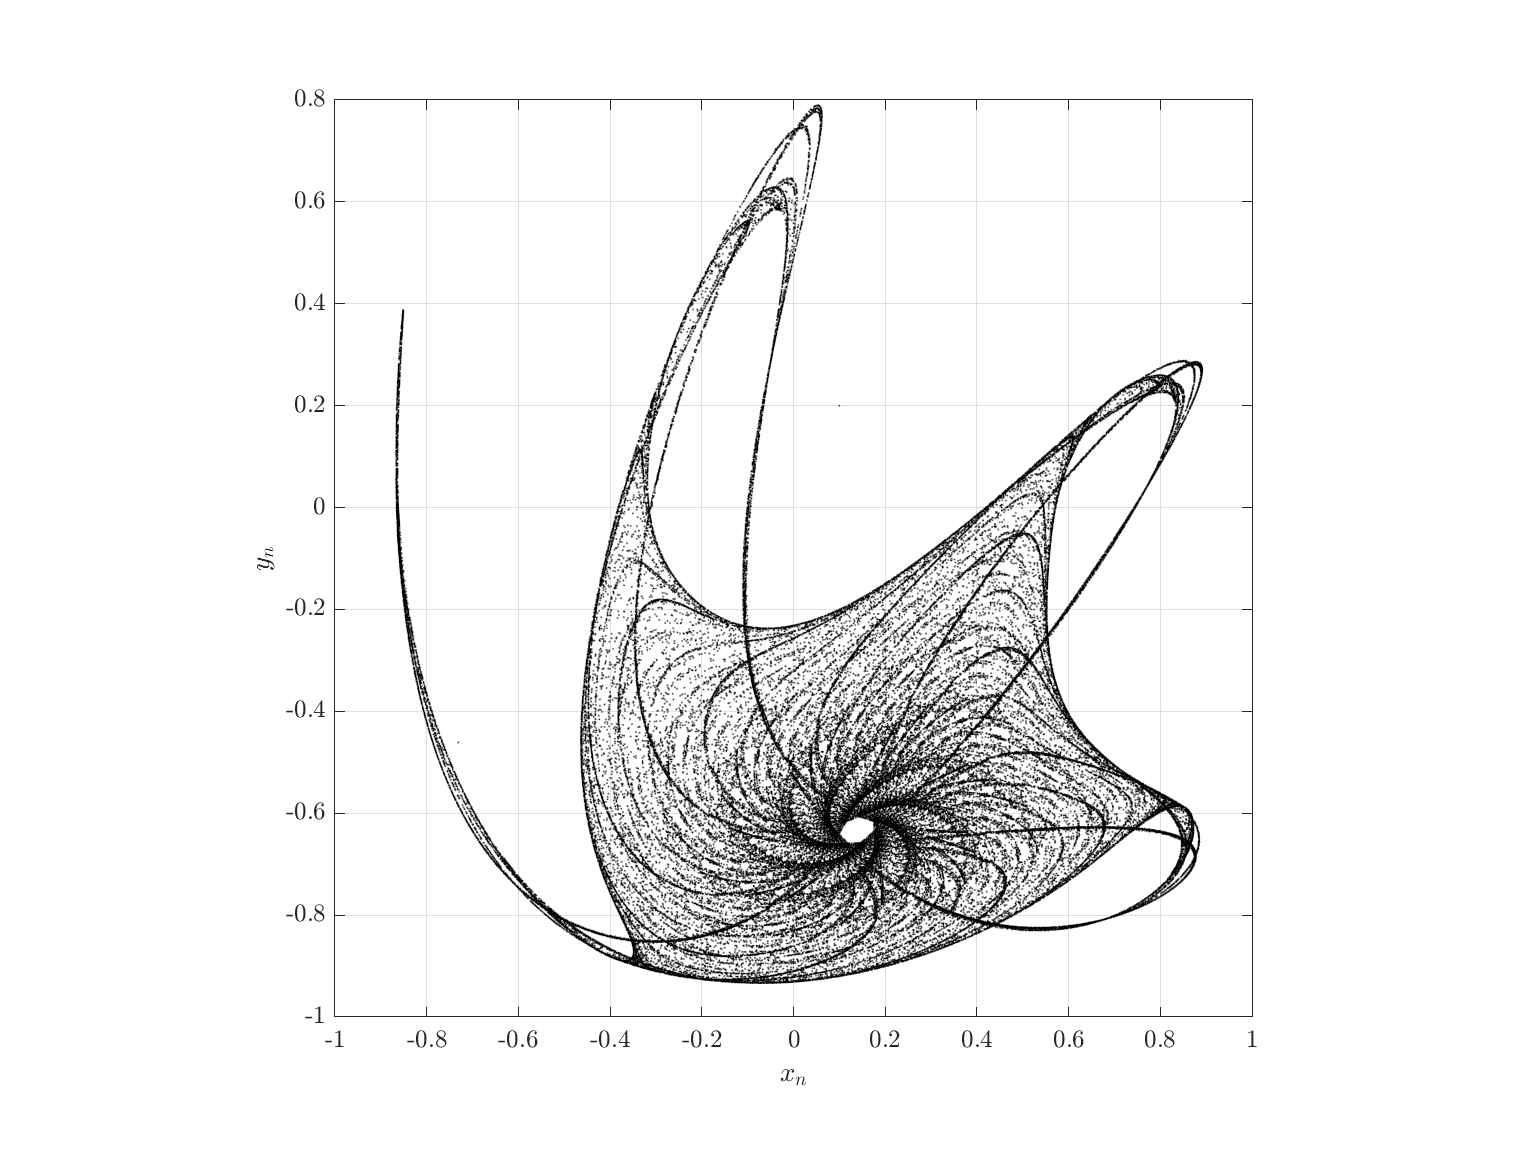
\includegraphics[width=\textwidth,trim=70 0 70 0,clip]{G1_map1}
                \caption{Atractor 1}    
                \label{fig:mapa_1}
            \end{subfigure}
            \hfill
            \begin{subfigure}[b]{0.475\textwidth}  
                \centering 
                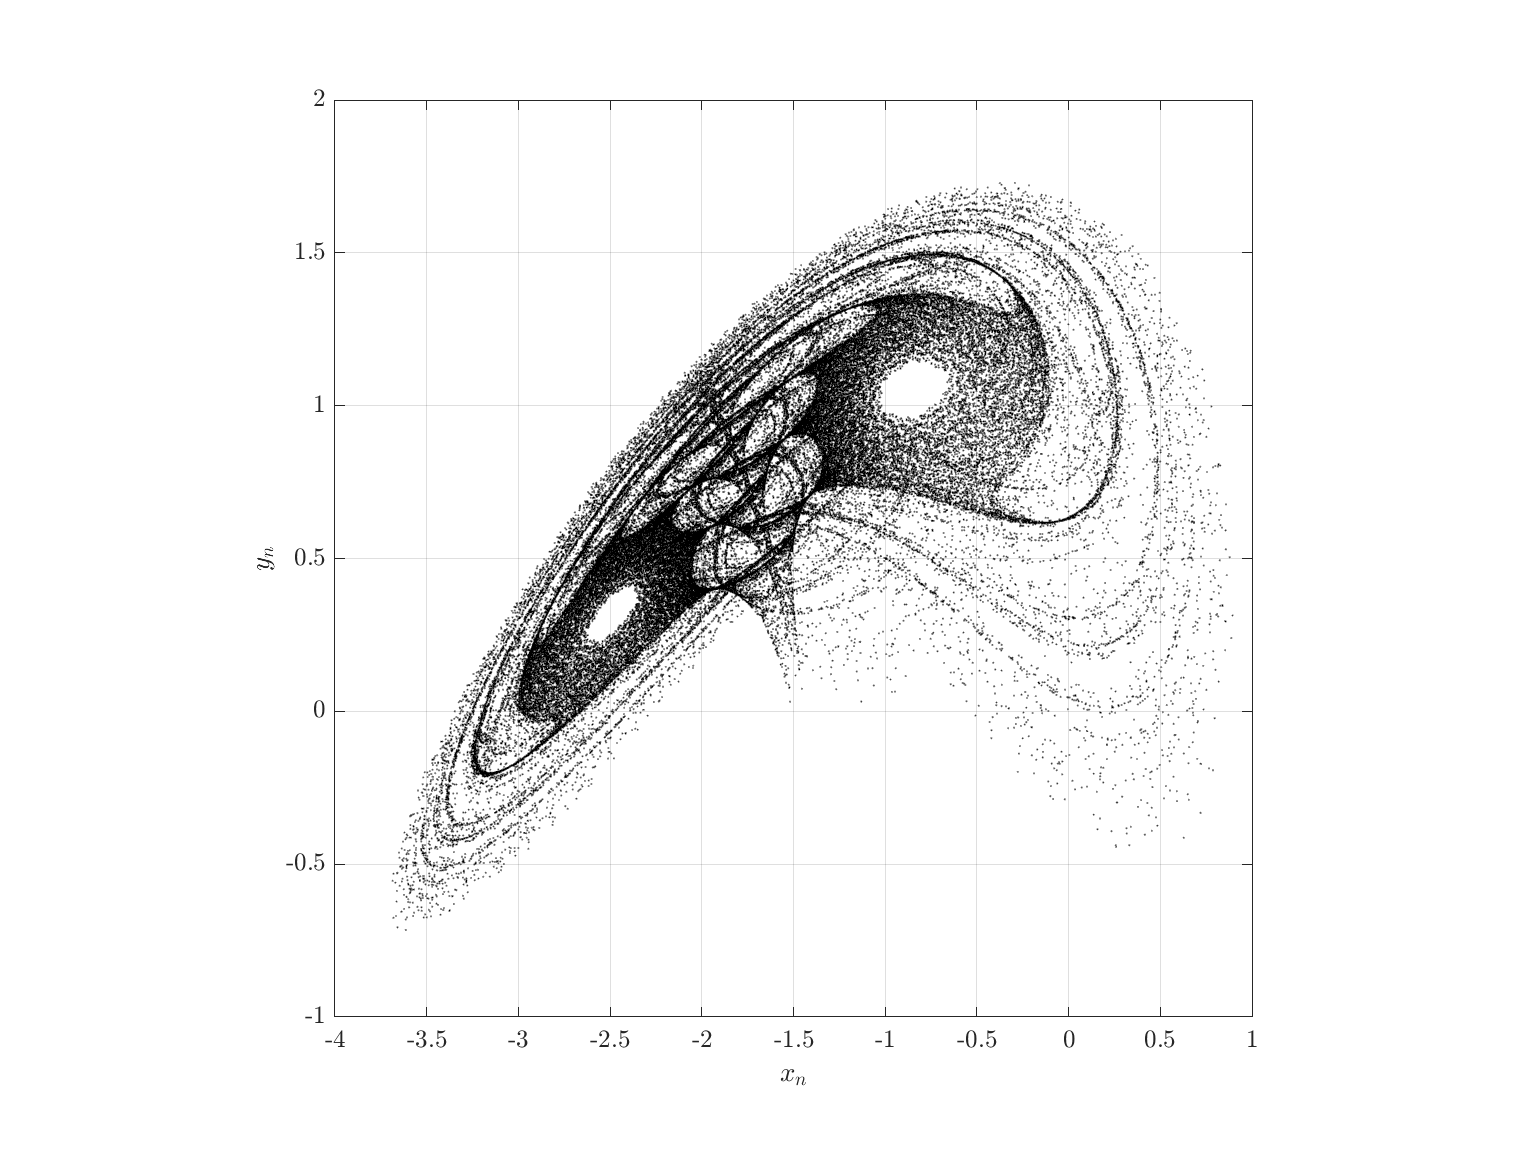
\includegraphics[width=\textwidth,trim=70 0 70 0,clip]{G2_map2}
                \caption{Atractor 2}    
                \label{fig:mapa_2}
            \end{subfigure}
            \vskip\baselineskip
            \begin{subfigure}[b]{0.475\textwidth}   
                \centering 
                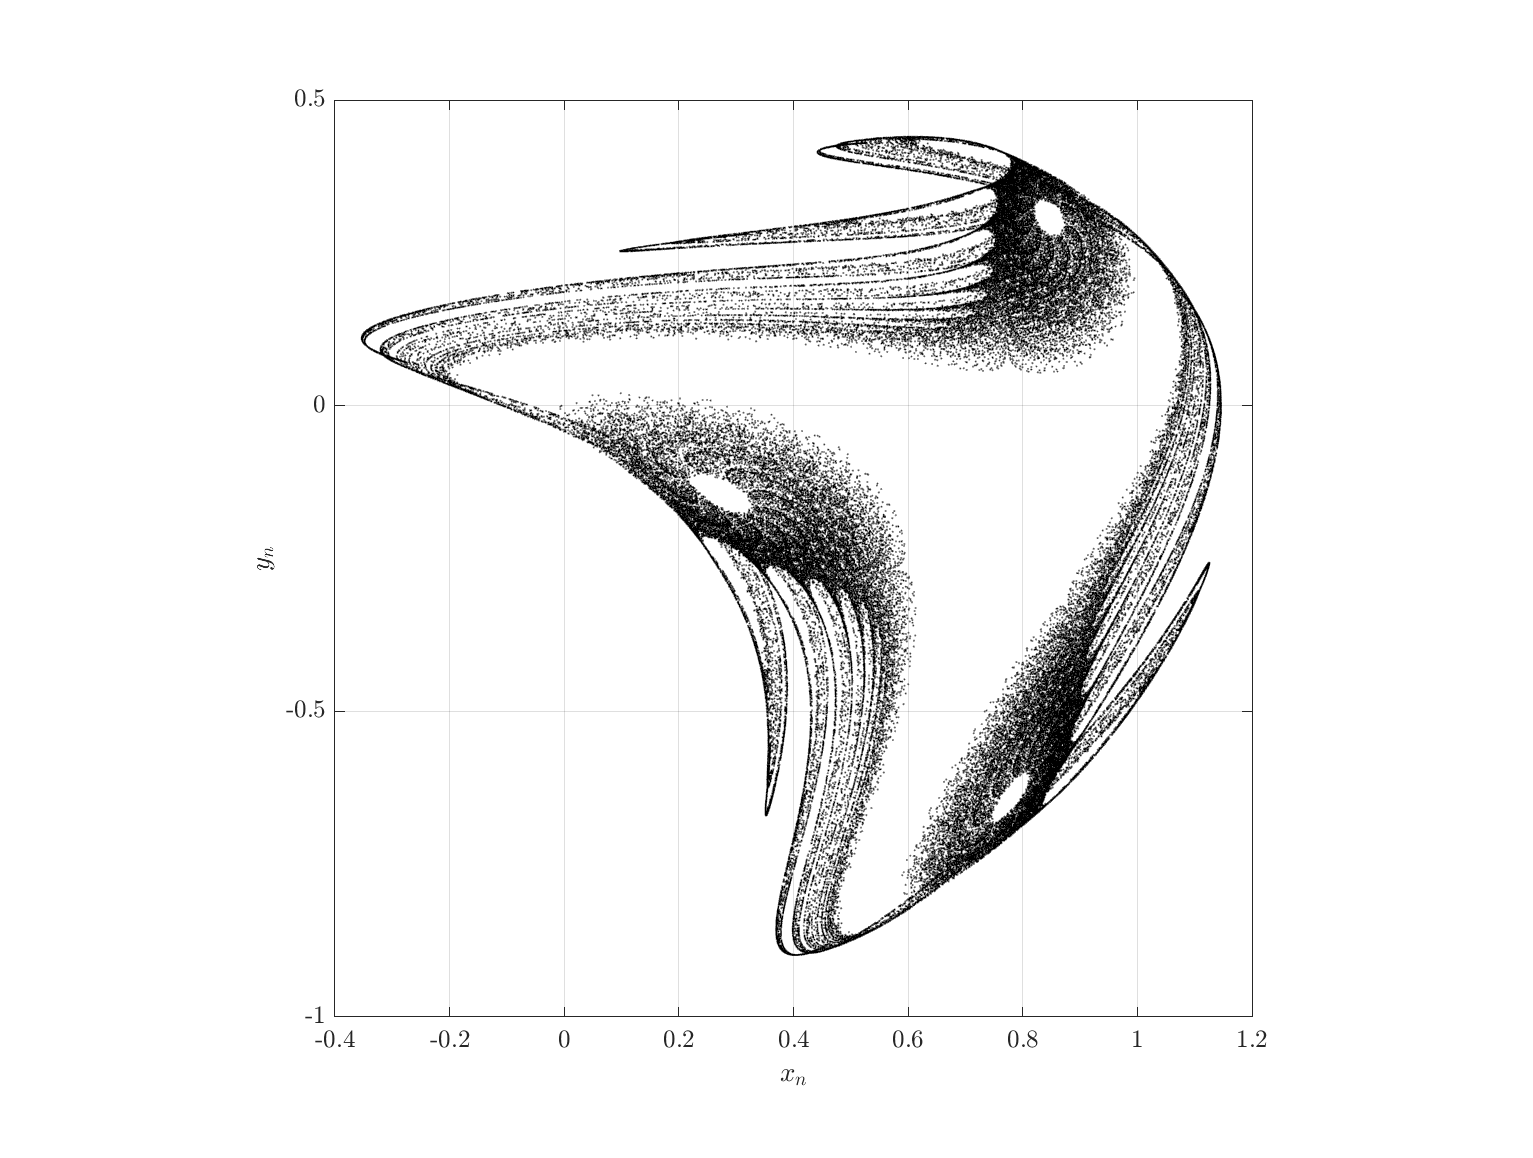
\includegraphics[width=\textwidth,trim=70 0 70 0,clip]{G3_map3}
                \caption{Atractor 3}    
                \label{fig:mapa_3}
            \end{subfigure}
            \hfill
            \begin{subfigure}[b]{0.475\textwidth}   
                \centering 
                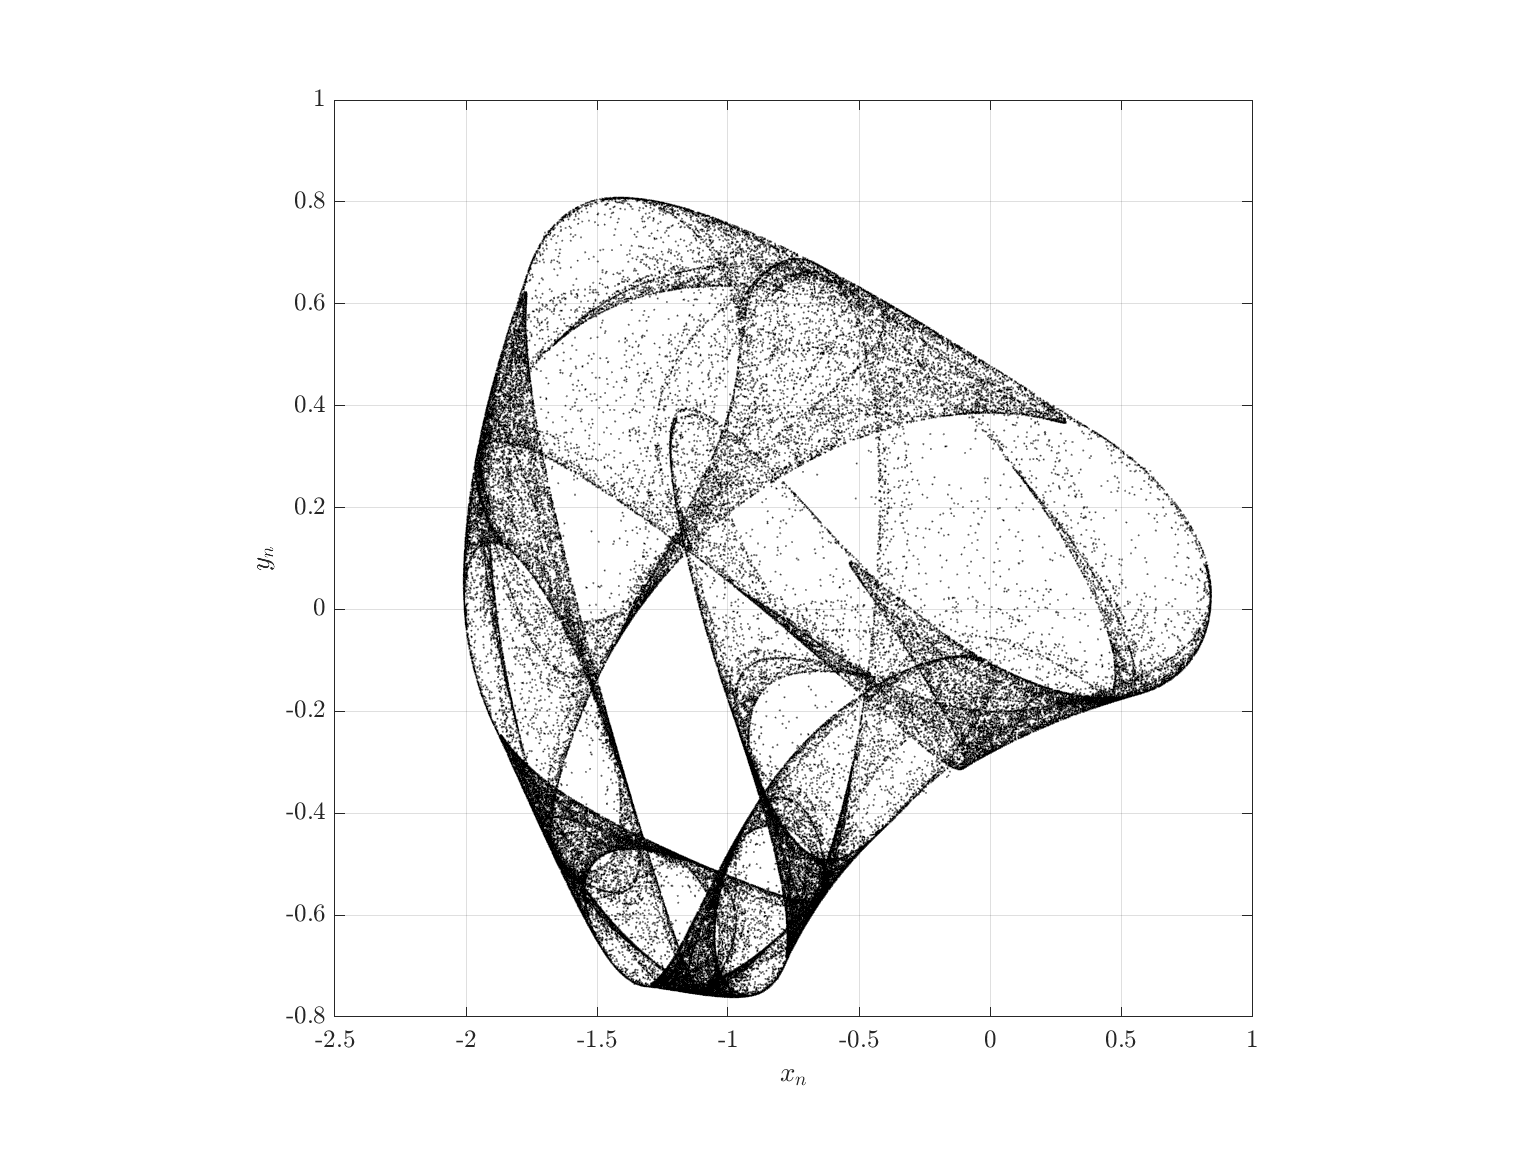
\includegraphics[width=\textwidth,trim=70 0 70 0,clip]{G4_map4}
                \caption{Atractor 4}    
                \label{fig:mapa_4}
            \end{subfigure}
            \vskip\baselineskip
            \begin{subfigure}[b]{0.475\textwidth}   
                \centering 
                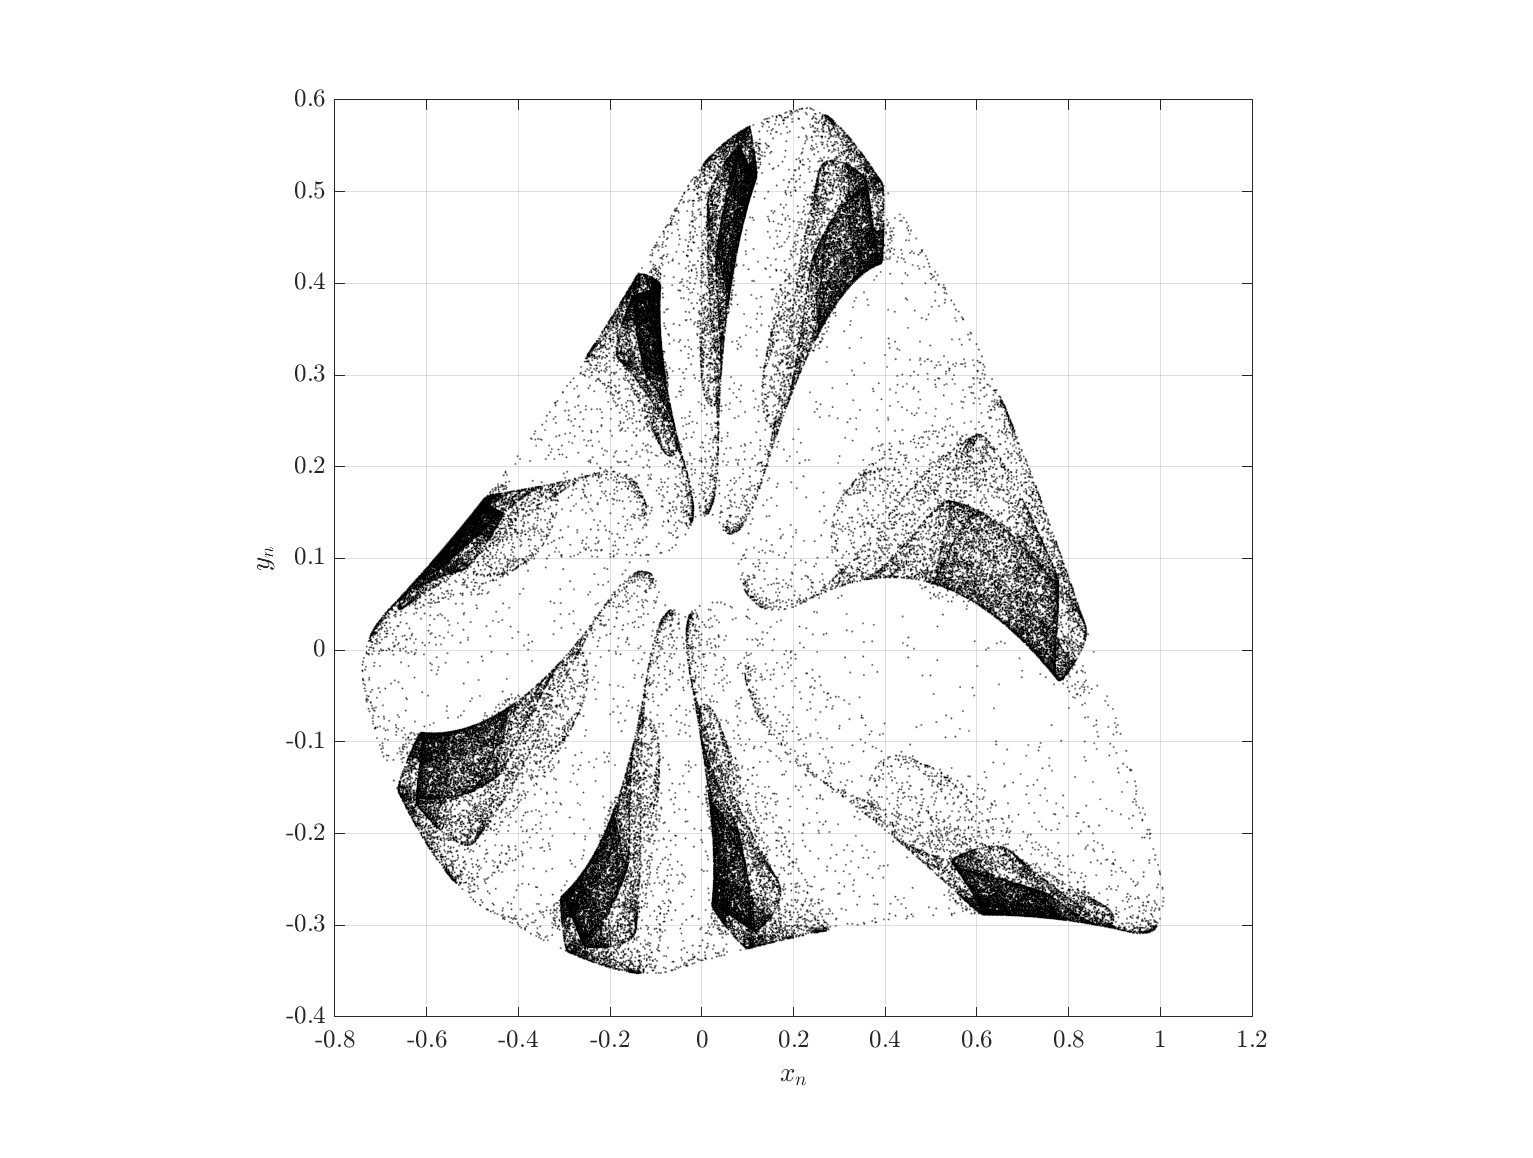
\includegraphics[width=\textwidth,trim=70 0 70 0,clip]{G5_map5}
                \caption{Atractor 5}    
                \label{fig:mapa_5}
            \end{subfigure}
            \hfill
            \begin{subfigure}[b]{0.475\textwidth}   
                \centering 
                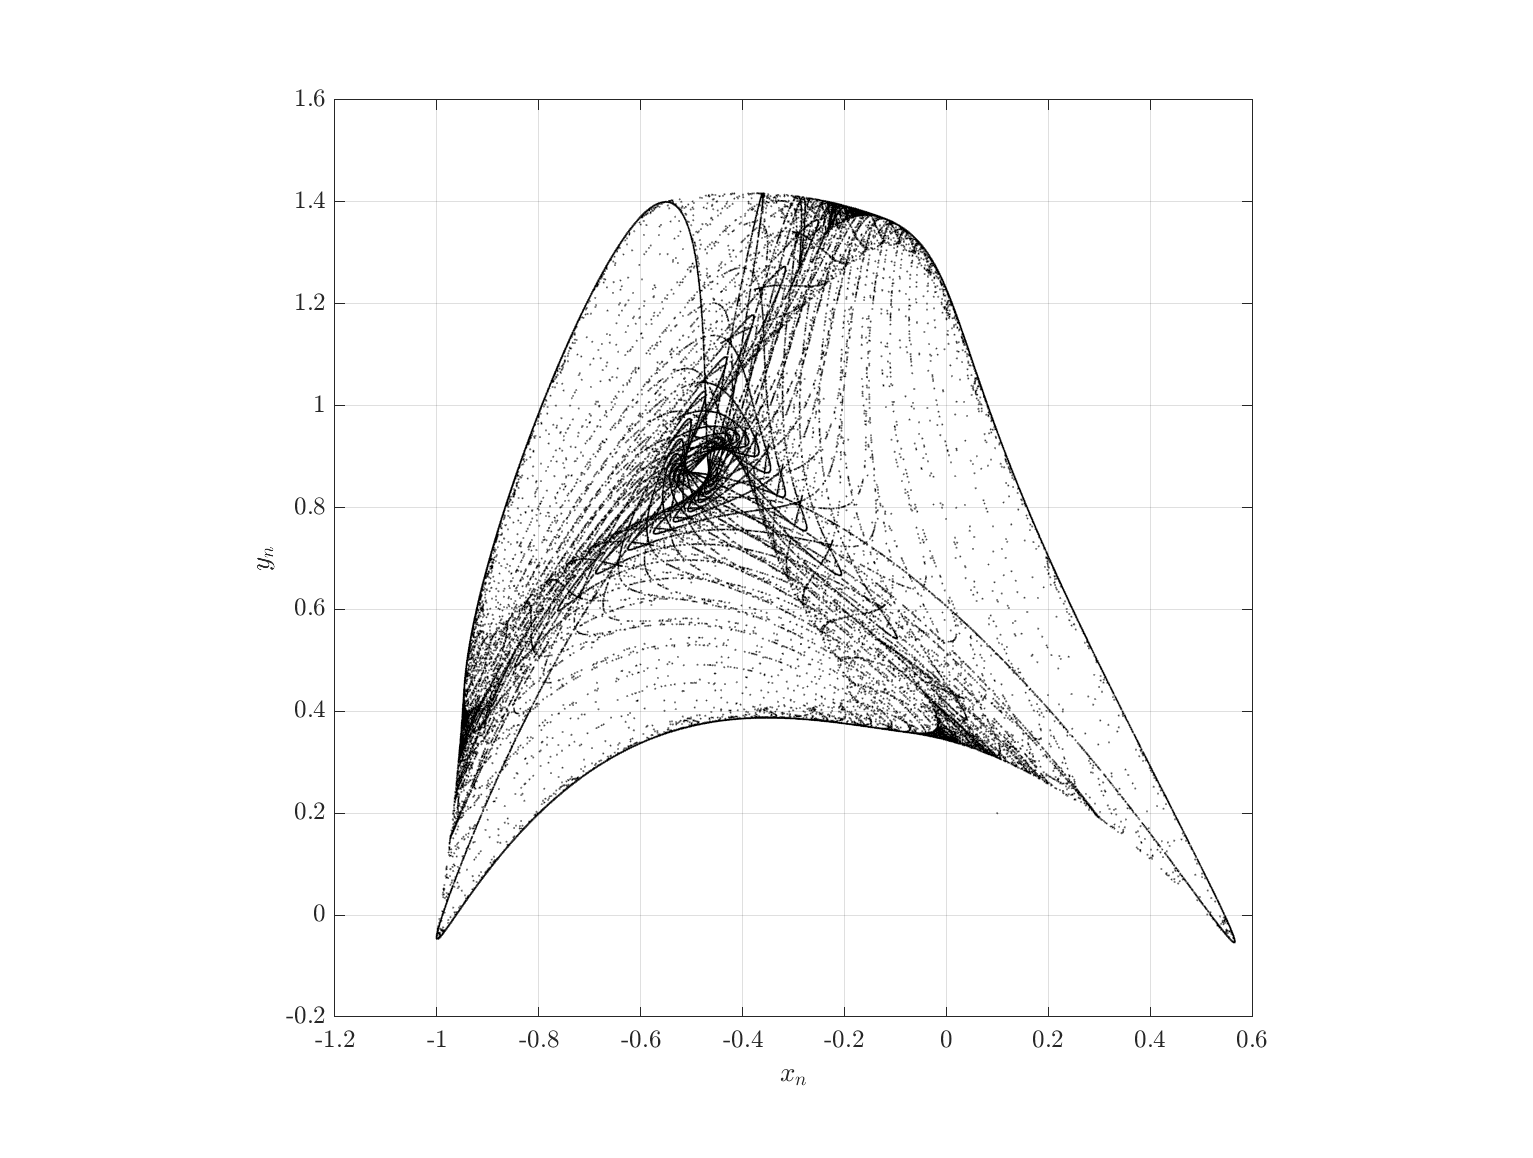
\includegraphics[width=\textwidth,trim=50 0 50 0,clip]{G6_map6}
                \caption{Atractor 6}    
                \label{fig:mapa_6}
            \end{subfigure}
            \caption{Diferentes atractores caóticos del mapa bidimensional generados en aritmética de punto flotante.} 
            \label{fig:multiples_atractores}
        \end{figure}

        Para resolver este problema se puede analizar el dominio de atracción que tienen cada uno de los mapas. Podemos calcularlo numéricamente siguiendo los siguientes pasos:

        \begin{enumerate}
            \item Elegir un rango para $x_{0} \in [x_{\text{izq}}, x_{\text{der}}]$ y $y_{0} \in [y_{\text{izq}}, y_{\text{der}}]$ y un tamaño de paso $h$ donde se va a realizar el análisis.
            \item Iterar el mapa unos cientos de veces para cada uno de los posibles valores de $x_{0}$ y $y_{0}$ dentro del rango y el tamaño de paso $h$ seleccionado. Para cada combinación almacenar todas las iteraciones en un vector.
            \item Comprobar cada vector en busca de puntos fijos, divergencia y de ser posible ciclos límite.
            \item En una matriz de tamaño, $m \times n$, donde $m$ es el número de elementos en el rango de $y_{0}$ y $n$ el número de elementos del rango de $x_{0}$, escribir 1 si esta dentro del rango que produce caos o $0$ si esta fuera.
        \end{enumerate}

       En la Figura \ref{fig:multiples_dominios} se muestran los dominios de atracción para cada uno de los mapas de la Tabla \ref{tab:codificacion} siguiendo el algoritmo anterior.

       Si analizamos los dominios de atracción de la Figura \ref{fig:multiples_dominios} podemos seleccionar un rango en el que sin importar cual sea la condición inicial existirá caos. Por comodidad seleccionaremos una ventana de 1 unidad tanto para $x_{0}$ como para $y_{0}$ como se muestran en la Tabla \ref{tab:rangos_mapas}. 

        \begin{table}[htbp]
            \centering
            \caption{Rangos usados para la condición inicial para cada uno de los atractores.}
            \begin{tabular}{|l|l|}
                \hline
                \rowcolor{lightgray} Atractor  & Rango de valores para $x_{0}$ y $y_{0}$ \\
                \hline
                $1$  & $x_{0} \in [-0.5, \phantom{-} 0.5]$, $y_{0} \in [-0.5, \phantom{-}0.5]$ \\
                \hline
                $2$  & $x_{0} \in [-1.0, \phantom{-} 0.0]$, $y_{0} \in [\phantom{-}0.0, \phantom{-}1.0]$ \\
                \hline
                $3$  & $x_{0} \in [\phantom{-}0.0, \phantom{-} 1.0]$, $y_{0} \in [-0.6, \phantom{-}0.4]$ \\
                \hline
                $4$  & $x_{0} \in [-1.5, -0.5]$, $y_{0} \in [-0.5, \phantom{-}0.5]$ \\
                \hline
                $5$  & $x_{0} \in [-0.4, \phantom{-}0.6]$, $y_{0} \in [-0.4, \phantom{-}0.6]$ \\
                \hline
                $6$  & $x_{0} \in [-1.0, \phantom{-}0.0]$, $y_{0} \in [\phantom{-}0.1, \phantom{-}1.1]$ \\
                \hline
            \end{tabular}
            \label{tab:rangos_mapas}
        \end{table}


        \begin{figure}[hbtp]
            \centering
            \begin{subfigure}[b]{0.475\textwidth}
                \centering
                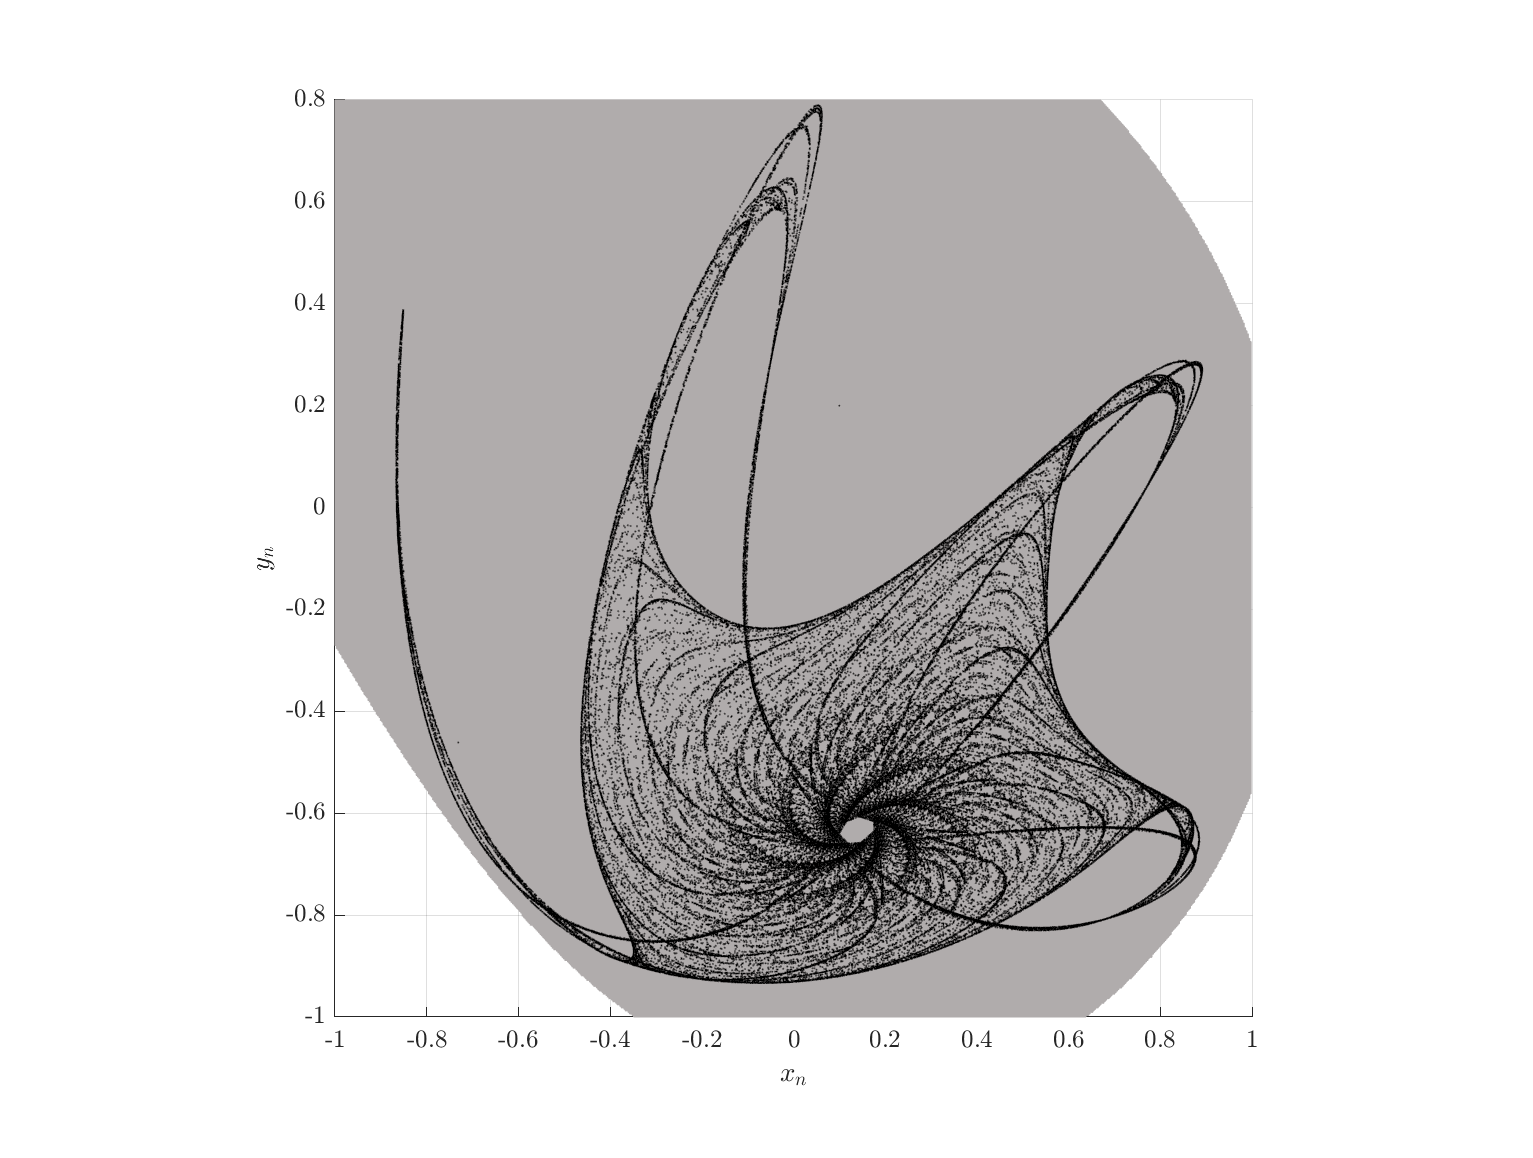
\includegraphics[width=\textwidth,trim=70 0 70 0,clip]{H1_map1}
                \caption{Atractor 1}    
                \label{fig:mapa_1h}
            \end{subfigure}
            \hfill
            \begin{subfigure}[b]{0.475\textwidth}  
                \centering 
                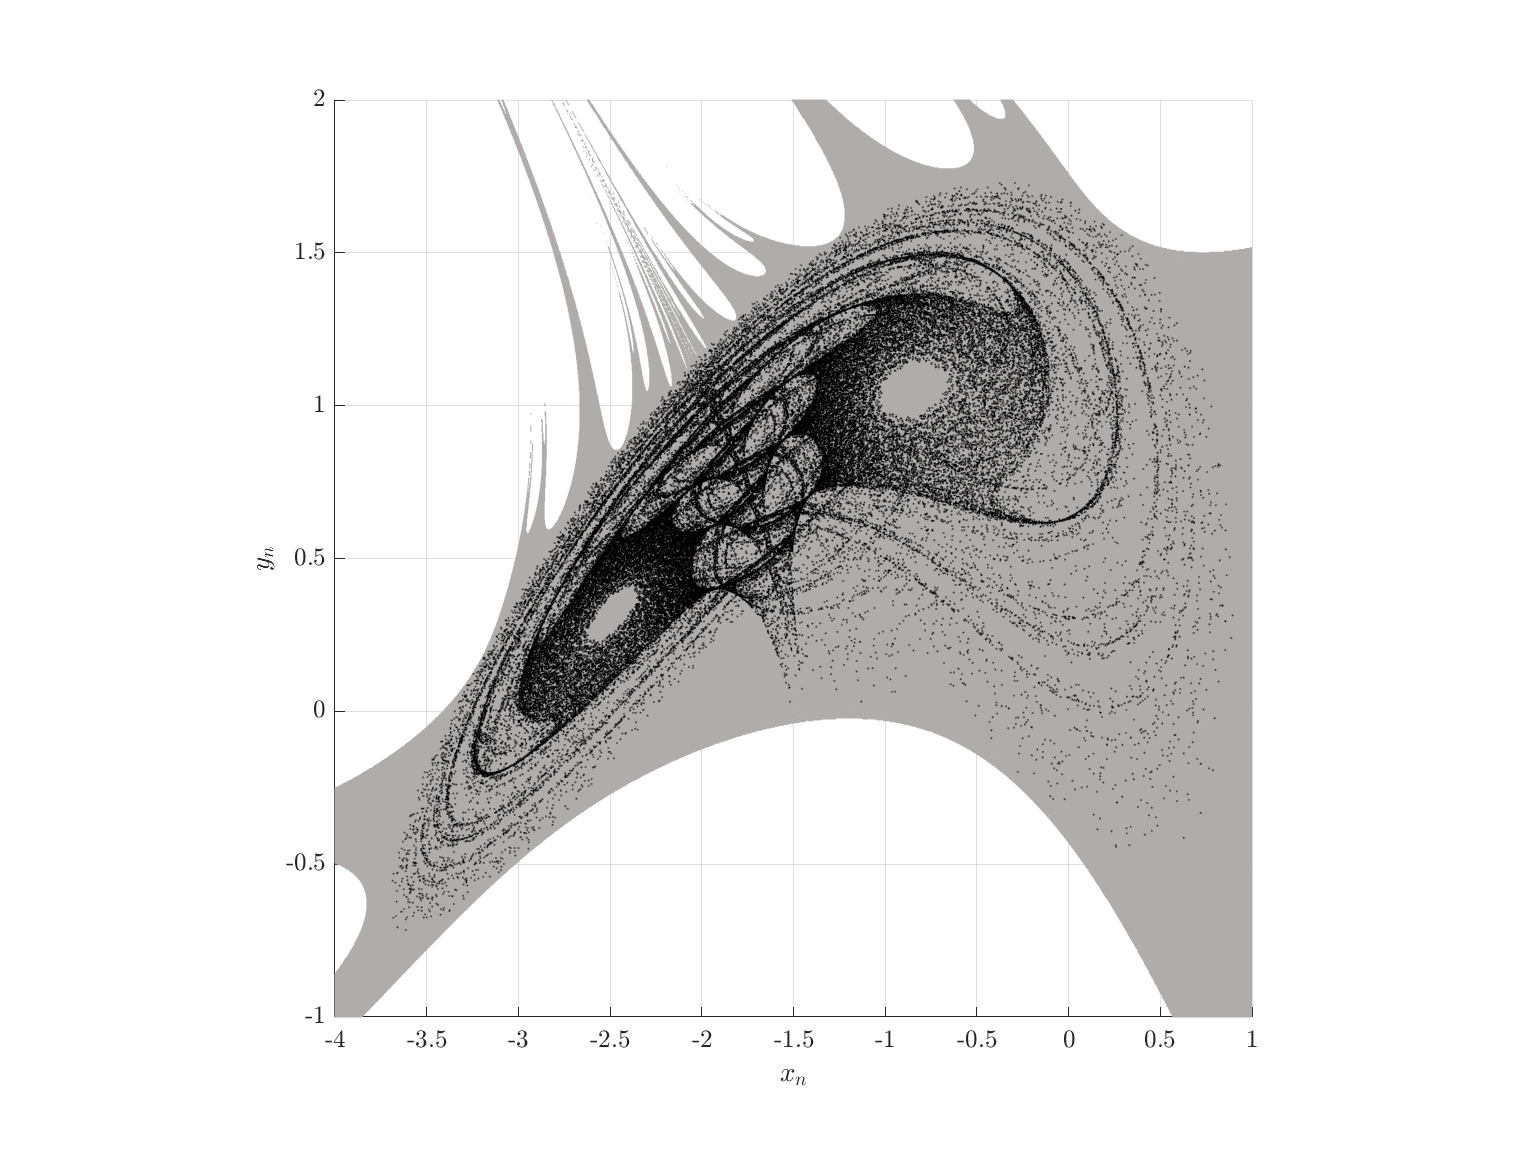
\includegraphics[width=\textwidth,trim=70 0 70 0,clip]{H2_map2}
                \caption{Atractor 2}    
                \label{fig:mapa_2h}
            \end{subfigure}
            \vskip\baselineskip
            \begin{subfigure}[b]{0.475\textwidth}   
                \centering 
                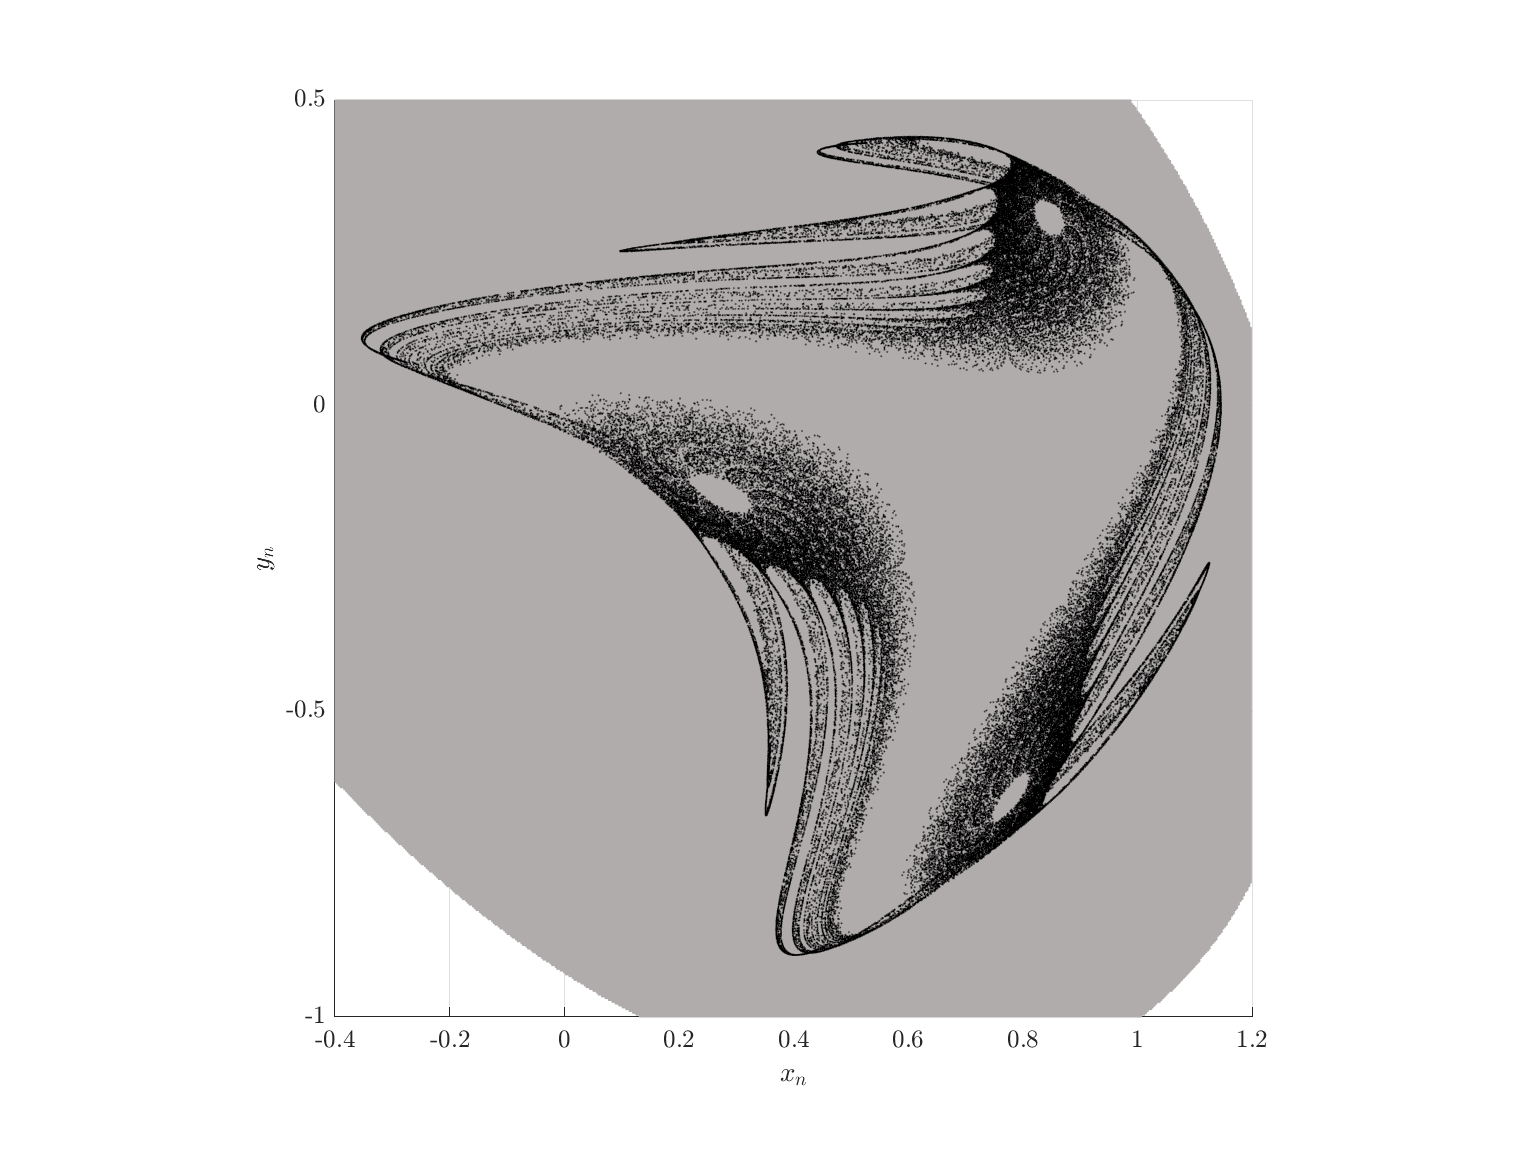
\includegraphics[width=\textwidth,trim=70 0 70 0,clip]{H3_map3}
                \caption{Atractor 3}    
                \label{fig:mapa_3h}
            \end{subfigure}
            \hfill
            \begin{subfigure}[b]{0.475\textwidth}   
                \centering 
                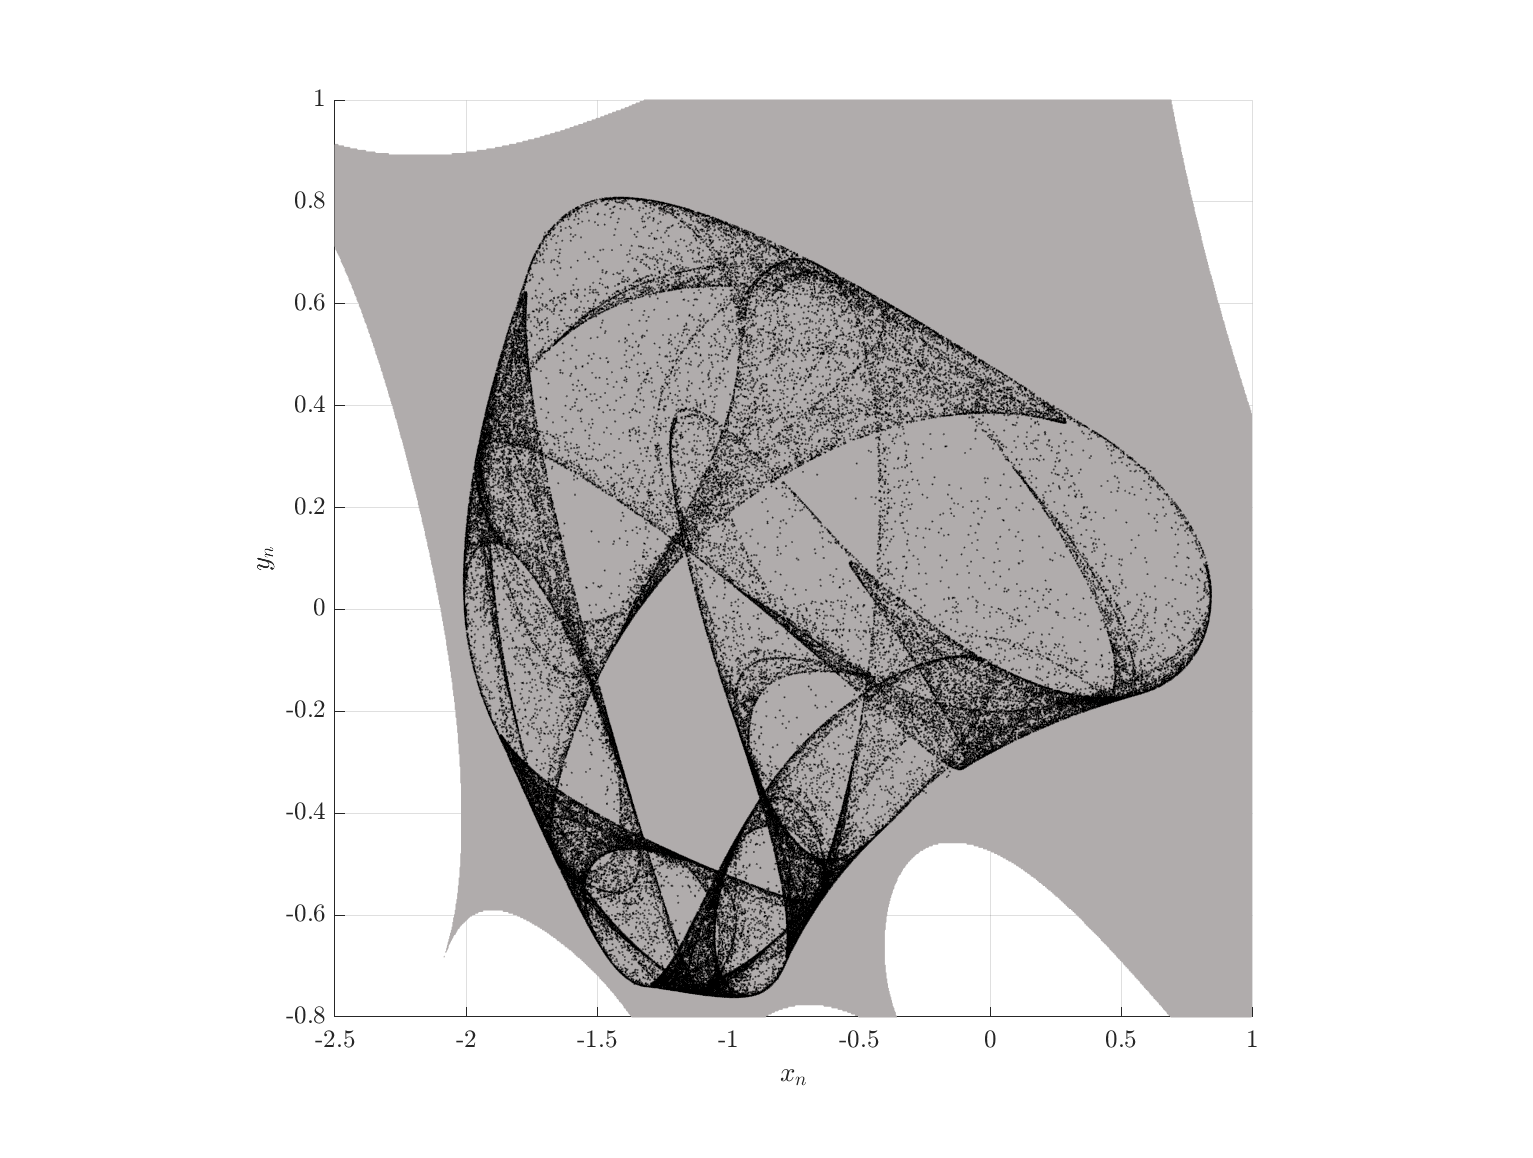
\includegraphics[width=\textwidth,trim=70 0 70 0,clip]{H4_map4}
                \caption{Atractor 4}    
                \label{fig:mapa_4h}
            \end{subfigure}
            \vskip\baselineskip
            \begin{subfigure}[b]{0.475\textwidth}   
                \centering 
                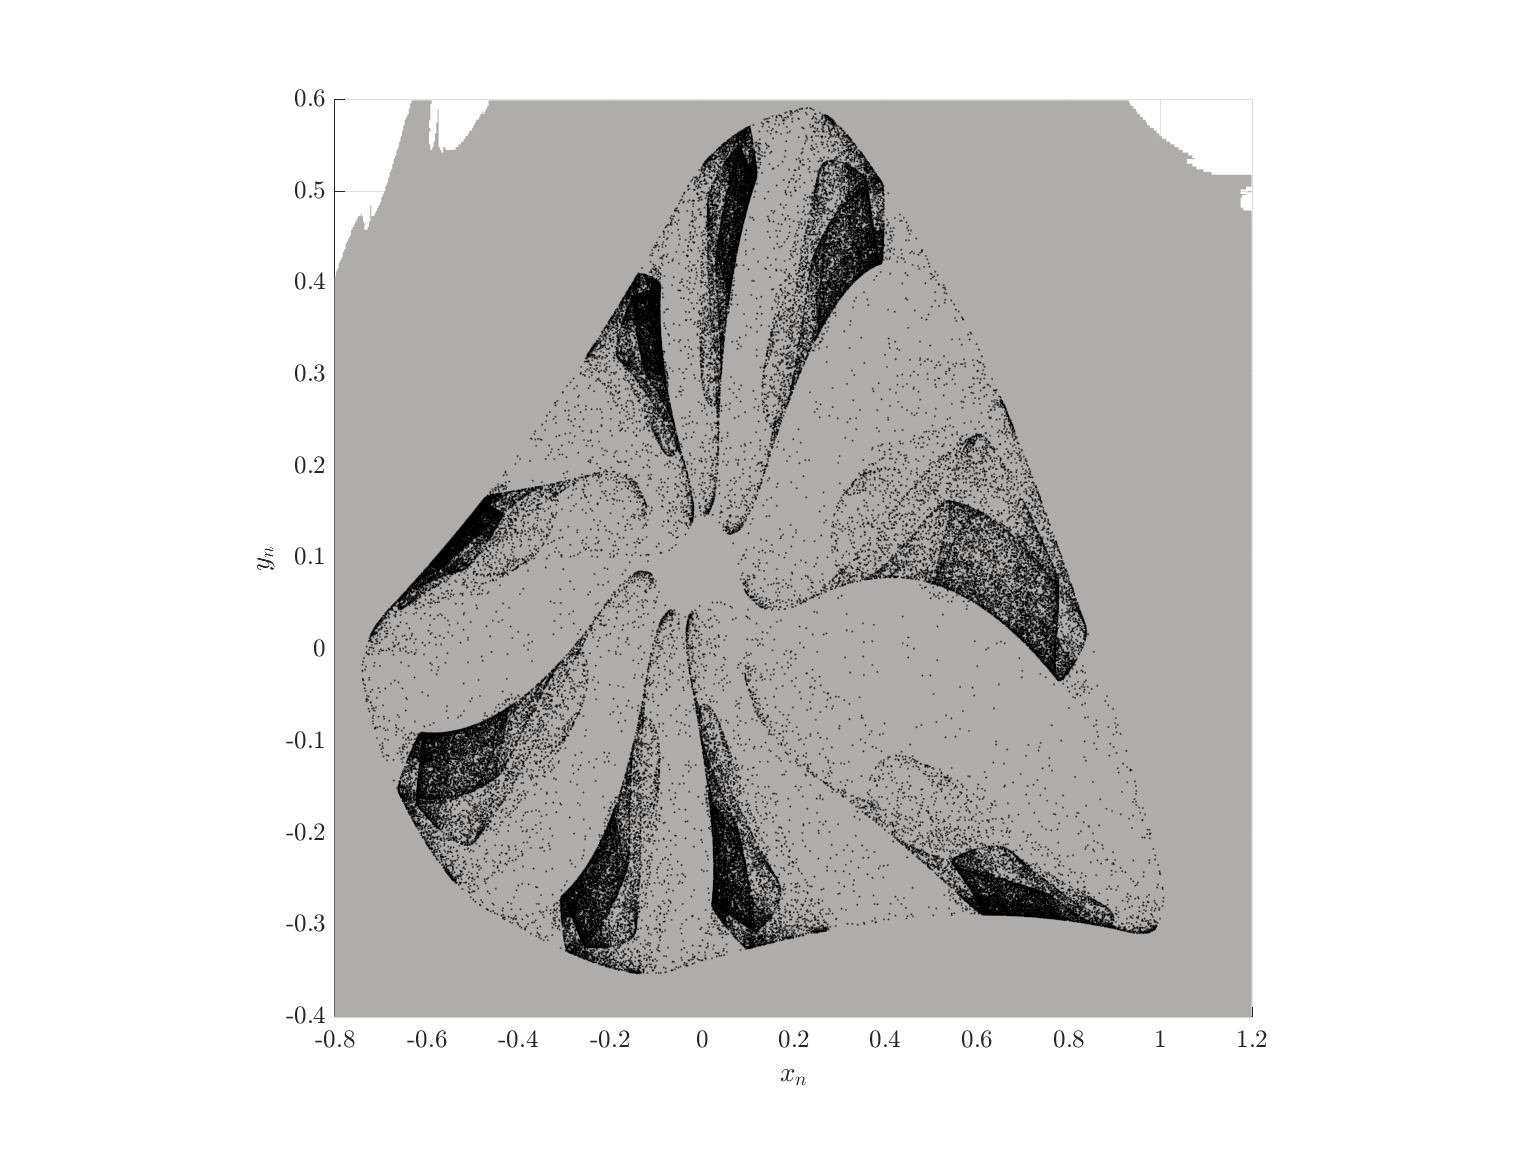
\includegraphics[width=\textwidth,trim=70 0 70 0,clip]{H5_map5}
                \caption{Atractor 5}    
                \label{fig:mapa_5h}
            \end{subfigure}
            \hfill
            \begin{subfigure}[b]{0.475\textwidth}   
                \centering 
                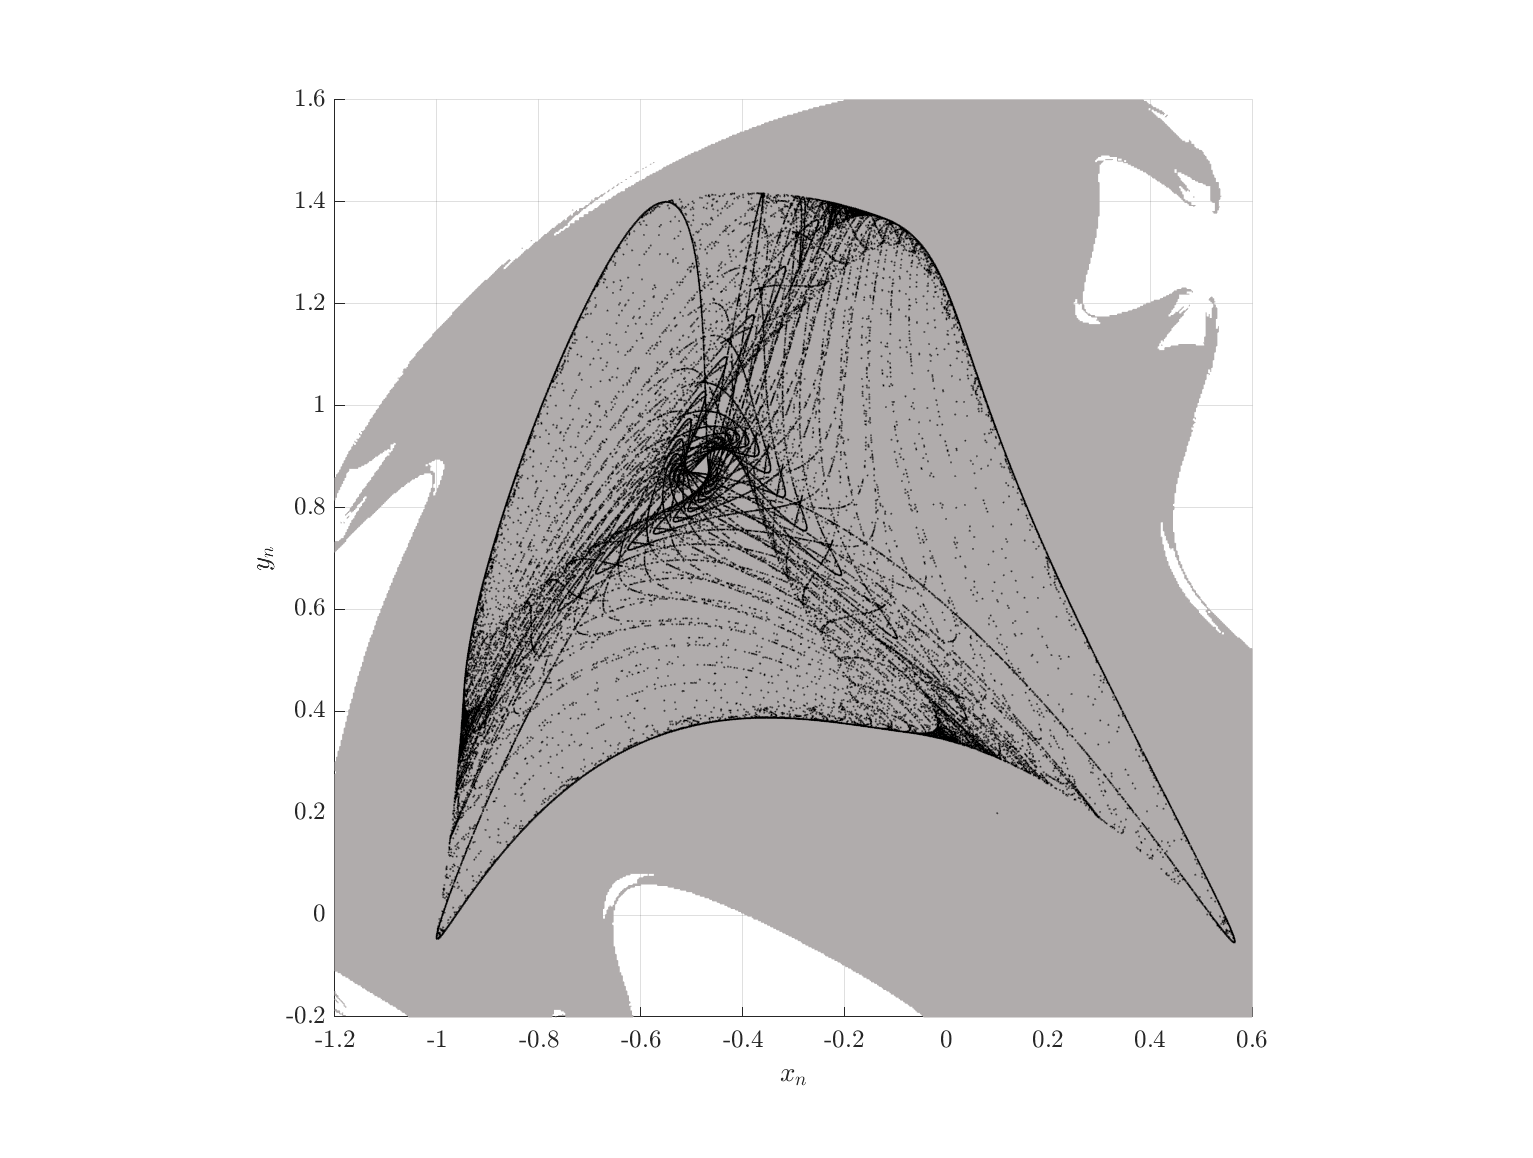
\includegraphics[width=\textwidth,trim=50 0 50 0,clip]{H6_map6}
                \caption{Atractor 6}    
                \label{fig:mapa_6h}
            \end{subfigure}
            \caption{Dominio de atracción de diferentes atractores caóticos del mapa bidimensional generados en aritmética de punto flotante.} 
            \label{fig:multiples_dominios}
        \end{figure}


        En \cite{Fraga2021} se utiliza el mapa caótico bidimensional propuesto en \cite{Sprott1993} y descrito en la ecuación (\ref{eq:mapa2d}) para diseñar un generador de números psedoaleatorios utilizando una arquitectura de punto fijo y extracción de bits haciendo uso de la operación mod 256 como se muestra en la ecuación (\ref{eq:extraccion}).

        \begin{equation}
            \begin{array}{lcl}
                s_{n+1} = \{ x_{n+1} \text{ mod } 256, y_{n+1} \text{ mod } 256 \}
            \end{array}
            \label{eq:extraccion}
        \end{equation}

       Asimismo se enfoca en utilizar solo los primeros 4 atractores que tienen los siguientes valores decodificados de la Tabla \ref{tab:codificacion}.

          \begin{equation*}
             \begin{array}{lcl}
                A_{1} & = & \{ -0.6, -0.1, \phantom{-}1.1, \phantom{-}0.2, -0.8, \phantom{-}0.6, -0.7, \phantom{-}0.7, \phantom{-}0.7, \phantom{-}0.3, \phantom{-}0.6, \phantom{-}0.9 \}\\
                A_{2} & = & \{ -1.0, \phantom{-}0.9, \phantom{-}0.4, -0.2, -0.6, -0.5, \phantom{-}0.4, \phantom{-}0.7, \phantom{-}0.3, -0.5, \phantom{-}0.7, -0.8 \}\\
                A_{3} & = &  \{\phantom{-}0.8, \phantom{-}1.0, -1.2, -1.0, \phantom{-}1.1, -0.9, \phantom{-}0.4, -0.4, -0.6, -0.2, -0.5, -0.7 \}\\
                A_{4} & = & \{-0.6, -0.4, -0.4, -0.8, \phantom{-}0.7, \phantom{-}0.3, -0.4, \phantom{-}0.4, \phantom{-}0.5, \phantom{-}0.5, \phantom{-}0.8, -0.1 \}\\
            \end{array}
        \end{equation*}

        En este trabajo utilizaremos un enfoque similar para crear un generador de números aleatorios híbrido.

    \section{Análisis de punto fijo}

        Una vez definido el sistema y los atractores a utilizar hay que seleccionar el formato de punto fijo óptimo para cada atractor. Como ejemplo utilizaremos el Atractor 1. Podemos notar que el Atractor 1 esta acotado en un rango de $x_{n} \in [-0.866, 0.8915]$ y $y_{n} \in [-0.933, 0.7896]$. Si echamos un vistazo a la ecuación (\ref{eq:mapa2d}), que por comodidad se vuelve a mostrar abajo, podemos notar que la operaciones que pueden generar los números con magnitud más grandes son la combinación de alguna de las sumas. En cuanto a las multiplicaciones, debido a que la mayoría de los coeficientes $|a_{n}| < 1$, con la excepción de $a_{3}$, después de realizar la multiplicación por cualquiera de ellos el número se vuelve más pequeño.

        \begin{equation*}
            \begin{array}{ccl}
                x_{n+1} & = &  a_{1} + a_{2}x_{n} + a_{3}x_{n}^{2} + a_{4}x_{n}y_{n} + a_{5}y_{n} + a_{6}y_{n}^{2}\\
                y_{n+1} & = &  a_{7} + a_{8}x_{n} + a_{9}x_{n}^{2} + a_{10}x_{n}y_{n} + a_{11}y_{n} + a_{12}y_{n}^{2}
            \end{array}
            %\label{eq:mapa2d}
        \end{equation*}

        Si tomamos los valores extremo de los rangos de $x_{n}$ y $y_{n}$ y analizamos las combinaciones de sumas que puedan generar el número más grande, o más pequeño en $x_{n+1}$ y $y_{n+1}$, al cual llamaremos $\beta$, podemos encontrar la cantidad de bits necesaria para la parte entera $a$ de la siguiente manera:

        \begin{equation}
                a = \log_{2} ( \text{abs}( \beta ) )
            \label{eq:bits_enteros}
        \end{equation}

       No obstante dependiendo el orden de las operaciones este análisis puede ser impreciso y solo nos da una aproximación del valor real de la parte entera. Consideremos lo siguiente, si se realizan primero todas las multiplicaciones y posteriormente se realizan las sumas, la acumulación de la suma puede ser mayor si se suman consecutivamente 3 números positivos a diferencia de intercalar números positivos con negativos.
       
       Otra cosa a considerar es la cantidad de bits fraccionarios $b$ que se requieren para que exista el caos. Si se tiene poca precisión en las operaciones la acumulación del error puede provocar que el caos solo exista por un corto periodo de tiempo. 

       Debido a lo anterior muchos diseñadores optan por elegir el formato de punto fijo a prueba y error. 

    \section{Simulador de arquitecturas digitales en C}

        Para no tener que recurrir al método de prueba y error para elegir el formato de punto fijo, en este trabajo se diseño un simulador de punto fijo en lenguaje C para poder comprobar la factibilidad de la arquitectura antes de pasar al diseño en hardware en FPGA. 

         La idea fundamental detrás de simular los diseños digitales en C antes de realizar su descripción en VHDL o Verilog es poder comprobar que las arquitecturas, ya sean de 16, 32 o 64 bits utilizando aritmética de punto fijo, funcionen correctamente desde el punto de vista de diseño, esto deja únicamente la posibilidad de cometer errores de sintaxis en el código en HDL los cuales se pueden analizar y solucionar por separado.

        Se utilizó el compilador de GCC versión 11.2.0 en una plataforma x64 en Linux. El tipo de dato es el primer punto fundamental para el simulador. Existen diversos tipos de datos en lenguaje C sin embargo para arquitecturas con tamaños de bits definidos podemos reducirlo a cuatro: \verb|__int128|, \verb|long|, \verb|int|, \verb|short|. Cada uno de estos tipos dato tiene una cantidad definida de bytes asociados dependiendo de la computadora y el compilador, para revisar la cantidad de bytes podemos utilizar el Código \ref{cod:A1} del Apéndice A. La salida del código se muestra en la Tabla \ref{tab:tipos_de_datos}.

        \begin{table}[htbp]
            \centering
            \caption{Tamaños de tipos de datos en C, compilador de GCC versión 11.2.0 en una plataforma x64 en Linux.}
            \begin{tabular}{|l|l|l|l|}
                \hline
                \rowcolor{lightgray} Tipo  & Bytes & Bits & Caracteres en hexadecimal\\
                \hline
                \verb|char|      & 1  & 8    & 2  \\
                \hline
                \verb|short|     & 2  & 16   & 4  \\
                \hline
                \verb|int|       & 4  & 32   & 8  \\
                \hline
                \verb|long|      & 8  & 64   & 16 \\
                \hline
                \verb|__int128|  & 16 & 128  & 32 \\
                \hline
            \end{tabular}
            \label{tab:tipos_de_datos}
        \end{table}
       
       Primero se simuló el Atractor 1 de la ecuación (\ref{eq:mapa2d}) en punto flotante para tener una referencia de los posibles valores de salida, en el Código \ref{cod:A2} se muestra esta simulación. Posteriormente se simuló el mapa tomando como punto de partida una arquitectura de 64 bits para tener suficiente precisión. El análisis de punto fijo arrojó una parte entera aproximada $a = 1$, con esta parte entera el sistema funciona sin problemas, sin embargo para los otros atractores es necesario utilizar una mayor cantidad de bits para la parte entera. En la Tabla \ref{tab:bits_atractores} se muestran los formatos seleccionados para cada atractor.
  
         \begin{table}[htbp]
            \centering
            \caption{Número de bits usados en la implementación de cada uno de los atractores con aritmética de punto fijo.}
            \begin{tabular}{|l|l|l|l|l|}
                \hline
                \rowcolor{lightgray} Atractor  & Bits parte entera & Bits parte fraccionaria & Rango  & Precisión\\
                \hline
                1     & 3                   & 60   & $[-8.0, 8.0]$   & $8.6739 \times 10^{-19}$\\
                \hline
                2     & 4                   & 59   & $[-16.0, 16.0]$ & $1.7347 \times 10^{-18}$\\
                \hline
                3     & 4                   & 59   & $[-16.0, 16.0]$ & $1.7347 \times 10^{-18}$\\
                \hline
                4     & 3                   & 60   & $[-8.0, 8.0]$   & $8.6739 \times 10^{-19}$\\
                \hline
            \end{tabular}
            \label{tab:bits_atractores}
        \end{table}

     En el Código \ref{cod:A3} se muestra el diseño del simulador. Este cuenta con funciones para realizar la conversión de punto flotante a punto fijo, multiplicación en punto fijo con truncamiento y finalmente conversión de punto fijo a punto flotante. En la Figura \ref{fig:B0_chaotic_map} se muestra el resultado de la simulación en punto fijo del atractor. Ya sea con 1, 2 o 3 bits para la parte entera, el Atractor 1 se simuló para 1000 millones de iteraciones y este no se salió de la órbita caótica.

        \begin{figure}[h!]
            \caption{Simulación del mapa caótico en punto fijo, Atractor 1.}
            \centering
            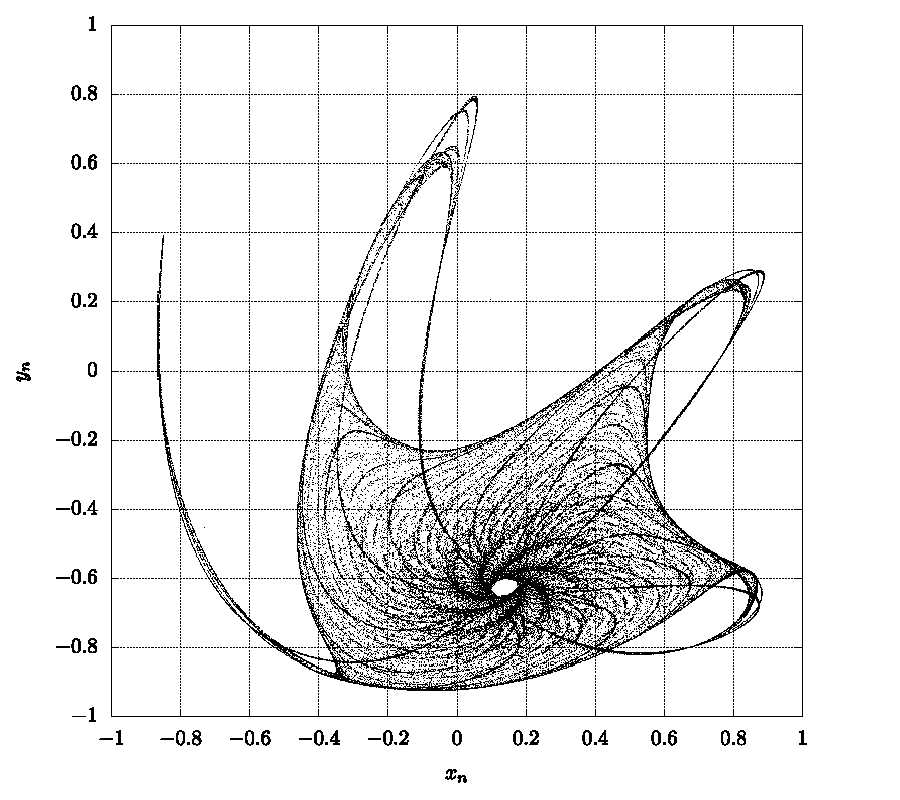
\includegraphics[width=0.8\linewidth]{B0_chaotic_map}
            \label{fig:B0_chaotic_map}
        \end{figure}

        Para simular la extracción de bits de la ecuación (\ref{eq:extraccion}) se pueden truncar los 8 bits menos significativos tanto para $x_{n}$ como para $y_{n}$ utilizando un casting del tipo \verb|unsigned char| como se muestra en el Código \ref{cod:A6} y para poder convertir la salida a binario se utilizó el Código \ref{cod:A7}.
        
        Simulando 100 millones iteraciones y generando palabras de 16 bits podemos ver la distribución de probabilidades de unos y ceros de cada palabra, en la Figura \ref{fig:J0_distribucion_exp} se muestra que la distribución es muy parecida a la ideal. Esto es lo esperado ya que los PRNG tienen por lo general buenas propiedades estadísticas.

        \begin{figure}[hbtp]
            \caption{Distribución de 100 millones de palabras de 16 bits.}
            \centering
            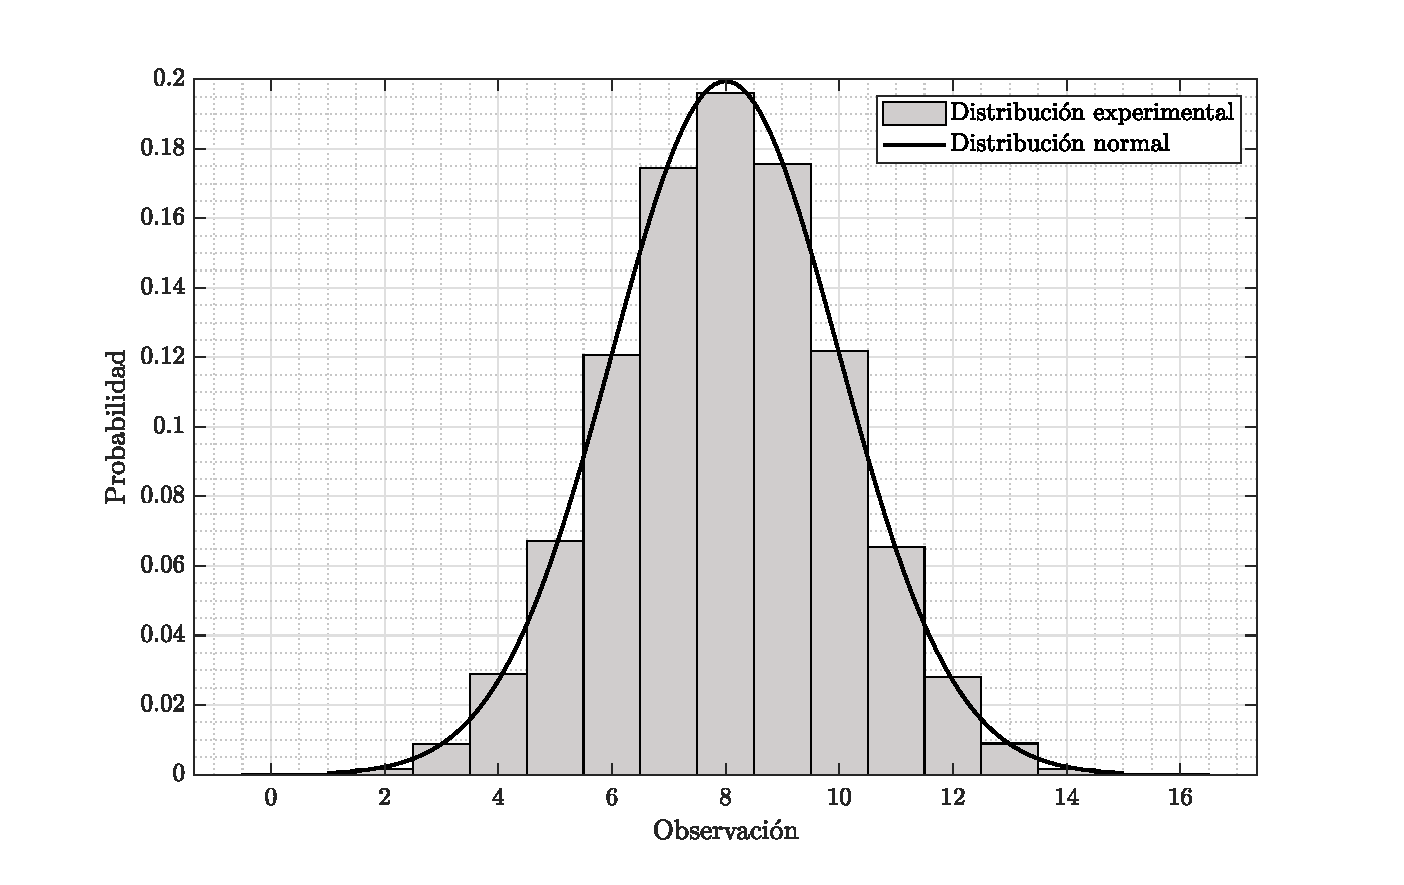
\includegraphics[width=0.8\linewidth]{J0_distribucion_exp}
            \label{fig:J0_distribucion_exp}
        \end{figure}

        Una vez comprobado el diseño con el simulador en C, visualizando tanto su atractor como su distribución de probabilidades normal podemos pasar con seguridad a la fase de descripción del sistema en hardware. En este trabajo se utilizó VDHL.

    \section{Diseño de mapa caótico en VHDL}

        Si analizamos la ecuación (\ref{eq:mapa2d}) podemos notar que su representación no es la más óptima para programarse en hardware, ya que se requieren 10 sumas y 16 multiplicaciones. No obstante si se reutilizan las multiplicaciones de $x_{n}^{2}$, $x_{n}y_{n}$ y $y_{n}^{2}$ solo se requieren 13 multiplicadores.

        Si reescribimos la ecuación (\ref{eq:mapa2d}) como se muestra en la ecuación (\ref{eq:mapaop}) se pueden eliminar dos multiplicadores más. Es decir la mínima cantidad de operaciones que se requieren para implementar el mapa son 10 sumadores y 11 multiplicadores.

        \begin{equation}
            \begin{array}{ccl}
                x_{n+1} & = &  a_{1} + ( a_{2} + a_{3}x_{n} )x_{n} + a_{4}x_{n}y_{n} + ( a_{5} + a_{6}y_{n} )y_{n} \\
                y_{n+1} & = &  a_{7} + ( a_{8} + a_{9}x_{n} )x_{n} + a_{10}x_{n}y_{n} + ( a_{11} + a_{12}y_{n})y_{n}
            \end{array}
            \label{eq:mapaop}
        \end{equation}

        Los bloques básicos para realizar la implementación serían: 
            
        \begin{enumerate}
            \item Un sumador de 64 bits con signo, Código \ref{cod:adder}.
            \item Un multiplicador de 64 bits con signo y truncamiento al formato de punto fijo especificado, Código \ref{cod:mult}.
            \item Una memoria ROM que almacene los valores en el formato de punto fijo de las constantes $a_{n}$, Código \ref{cod:rom_cm}.
            \item Un multiplexor para poder seleccionar entre la condición inicial y la retroalimentación del sistema, Código \ref{cod:mux_ic}.
            \item Un registro que almacene la iteración actual, Código \ref{cod:ff_hab}.
            \item Una máquina de estado para controlar todo el sistema, Código \ref{cod:fsm_cm}.            
        \end{enumerate}
    
        Visto como diagrama de bloques la implementación el sistema completo se muestra en la Figura \ref{fig:B1_architecture} y el Código de la implementación en \ref{cod:chaotic_map}.
        
        \begin{figure}[hbtp]
            \caption{Diagrama de bloques del mapa caótico.}
            \centering
            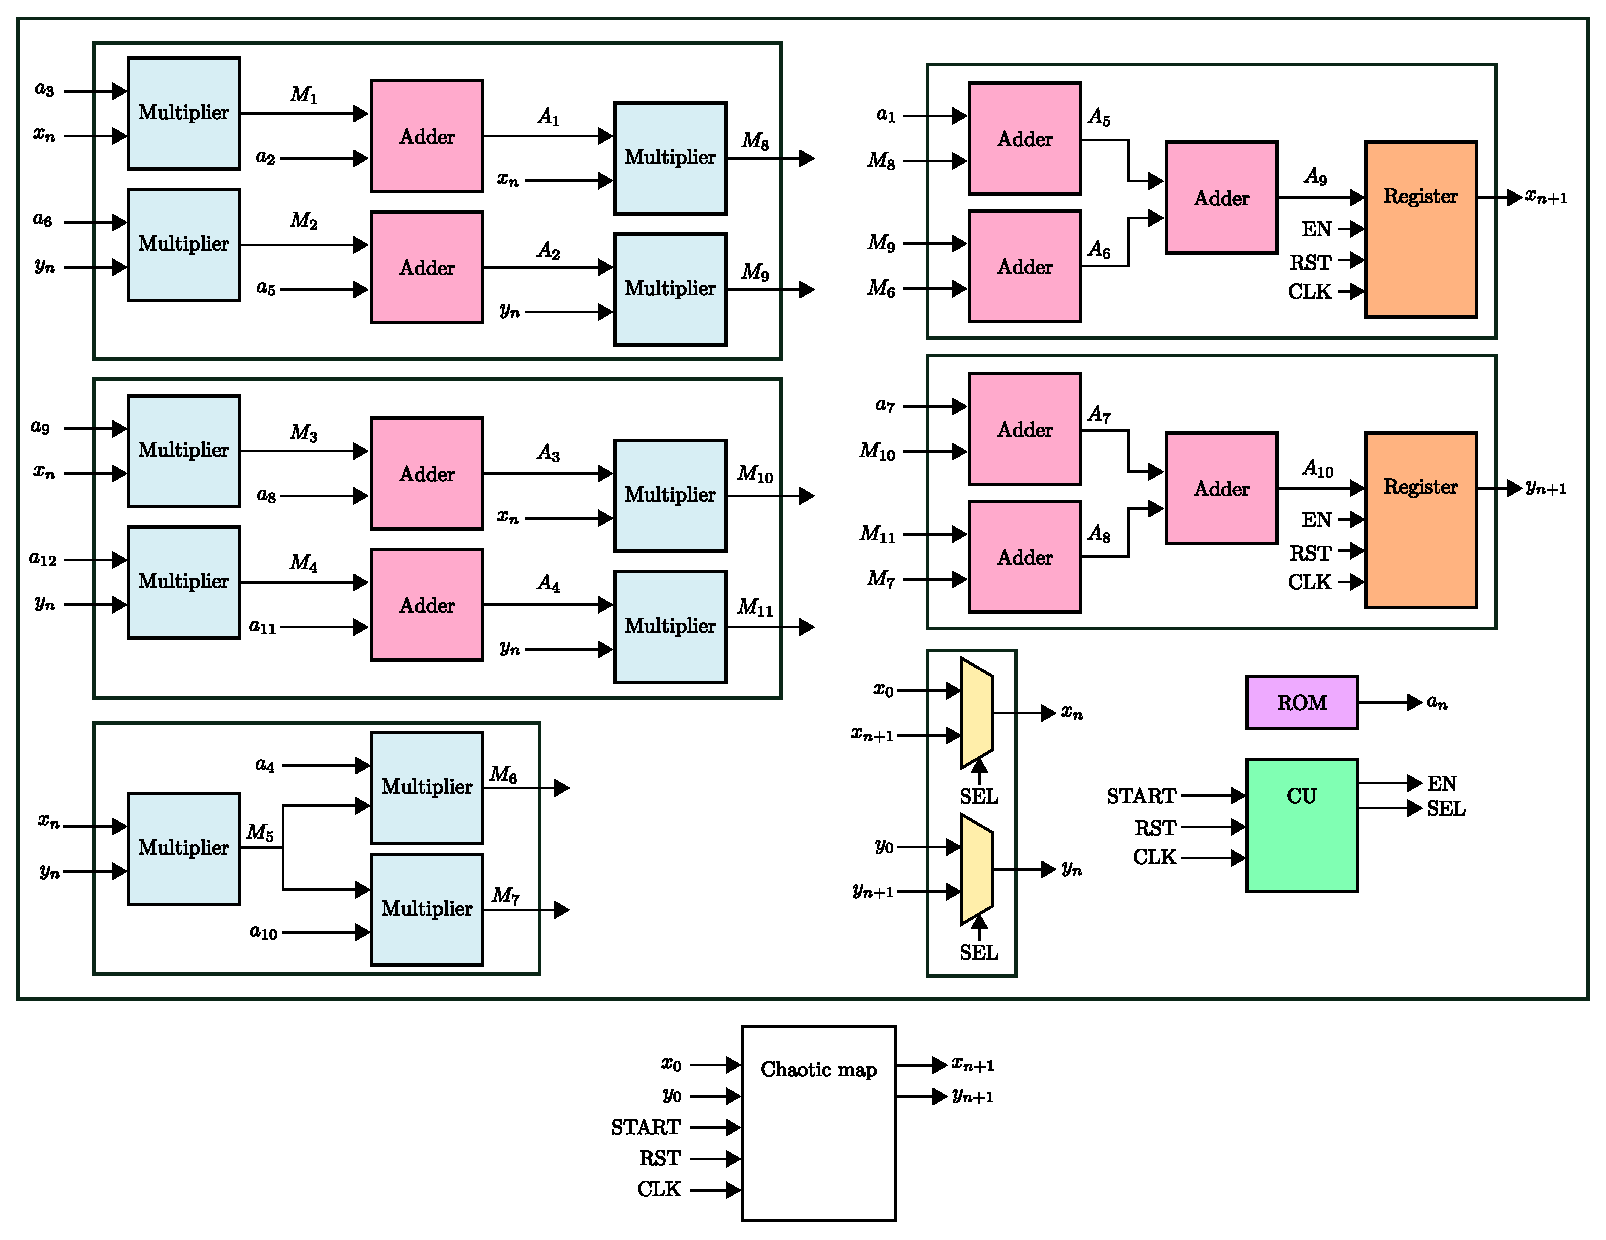
\includegraphics[width=0.9\linewidth]{B1_architecture}
            \label{fig:B1_architecture}
        \end{figure}

        En la Figura \ref{fig:B2_fsm_cm} se muestra la máquina de estados que controla al sistema. El estado $S_{0}$ tiene la función de seleccionar la condición inicial direccionando el multiplexor a partir de la señal EN y esperar a que la señal de inicio START ocurra. El estado $S_{1}$ mantienen el direccionamiento del multiplexor y habilita el registro de salida que almacena la iteración actual atreves de la señal EN. El estado $S_{2}$ es similar en funcionamiento el estado $S_{0}$ con la única diferencia que direcciona el multiplexor al registro de salida para formar un lazo de retroalimentación para las futuras iteraciones. Finalmente el estado $S_{3}$ mantiene el multiplexor direccionando la retroalimentación y habilita el registro de salida para almacenar la iteración actual. 

        \begin{figure}[hbtp]
            \caption{Máquina de estados de mapa caótico.}
            \centering
            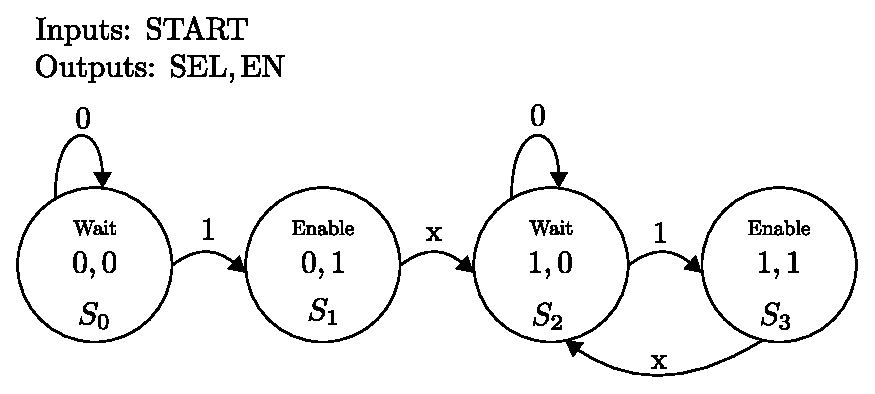
\includegraphics[width=0.6\linewidth]{B2_fsm_cm}
            \label{fig:B2_fsm_cm}
        \end{figure}


    \section{Multiplicador de una sola constante (SCM)}

        Es bien sabido que los multiplicadores son estructuras que consumen una gran cantidad de recursos en dispositivos digitales, por esto esta razón, es muy común que los diseñadores realicen optimizaciones creando multiplicadores de una sola constante para reducirlos.

        Al multiplicar por una constante conocida, podemos explotar las propiedades de la multiplicación binaria para obtener un circuito de hardware funcionalmente equivalente con menos recursos lógicos en comparación con conectar la constante en una entrada de un multiplicador genérico. La multiplicación constante puede implementarse como un conjunto de sumas, restas y desplazamientos binarios.

            En los términos sencillos, el problema de la multiplicación constante puede describirse del siguiente modo: Dado un conjunto de constantes $T$, encontrar una realización suma-resta-desplazamiento de $t \cdot x$ para cada $t \in T$ donde $x$ es una variable. El objetivo es minimizar el número de sumadores.
            
            Por ejemplo supongamos que $T = \{29 \}$, lo que significa que queremos implementar $29 \cdot x$. Una solución sería $29x = 32x - 4x +x = 2^{5} - 2^{2}x + x = (x \ll 5) - (x \ll 2) + x$ donde $ \ll n $ denota un desplazamiento a la izquierda de $n$ bits. Ver Figura \ref{fig:J1_scm}.

        \begin{figure}[hbtp]
            \caption{Ejemplo de multiplicación de una sola constante.}
            \centering
            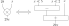
\includegraphics[width=0.6\linewidth]{J1_scm}
            \label{fig:J1_scm}
        \end{figure}
        
        En \cite{Thong2011} se propone un algoritmo óptimo y bastante práctico para poder crear multiplicadores de una constaste de manera sencilla. Se requieren solo la constante y el número de bits fraccionarios, no obstante esta restringido a arquitecturas de máximo 32 bits y máximo 25 bits para la parte fraccionaria.

        Se pueden crear a mano estos multiplicadores de una constante, no obstante encontrar una solución óptima para estos problemas es NP completo. NP es el conjunto de problemas en los que podemos comprobar en un tiempo razonable si una respuesta al problema es correcta o no y los problemas NP completos son los problemas más difíciles de todo NP. A grandes rasgos se buscan algoritmos que puedan resolver el problema de encontrar la solución de descomponer una multiplicación por una constante en sumas, restas y desplazamientos con la menor cantidad de recursos.

    Si se tienen más de un multiplicador otro tipo de optimización que se puede realizar es analizar cuales corrimientos se comparten entre multiplicadores de una constante y reutilizar los corrimientos.

    En este trabajo se diseñaron a mano multiplicadores de una constante para los parámetros $a_{n}$.

    \section{Diseño de generador de semillas}

        Hasta este punto, tenemos un mapa caótico implementado en FPGA capaz de generar números pseudoaleatorios en palabras de 16 bits cada dos ciclos de reloj. El problema es que las condiciones iniciales $x_{0}$ y $y_{0}$ son fijas, es decir, si algún atacante tuviera el conocimiento de las condiciones iniciales y conociera el mapa, este sería capaz de reproducir el sistema ya que el mapa por si mismo es determinista. Por esta razón se utiliza un TRNG para sembrar el generador de números pseudoaleatorios. Esto convierte al sistema en un generador de números aleatorios híbrido, aumenta la seguridad agregando una capa de complejidad y debido a que los TRNG extraen la aleatoriedad de elementos físicos, es muy difícil que alguien pueda adivinar las condiciones iniciales. 

        De todos los TRNG presentados en este trabajo el ERO-TRNG fue el candidato seleccionado para servir como generador de semillas. Este TRNG tiene una metodología bien estructurada, un modelo estocástico bien estudiado y sus propiedades tanto de entropía, uso de área y consumo de potencia son buenas. Además tiene la ventaja de ser el TRNG con mayor compatibilidad y su repetibilidad entre familias de FPGA. El diseño no requiere ninguna intervención manual para obtener resultados satisfactorios. 

        En la Figura \ref{fig:J2_trng} se muestra nuestra propuesta para extraer 64 bits aleatorios para generar la semilla del PRNG. Consiste en utilizar un registro de corrimiento a la derecha (RSR) que muestrear el ERO-TNG y comparar si los 64 bits extraídos se encuentran dentro del rango del dominio de atracción del mapa caótico utilizando los parametros del Atractor 1. Un contador de 5 bits de una sola vuelta asegura que se hayan generado 64 bits y no pasé una semilla incompleta.

        \begin{figure}[hbtp]
            \caption{Generador de semilla.}
            \centering
            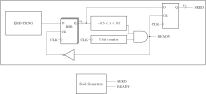
\includegraphics[width=0.8\linewidth]{J2_trng}
            \label{fig:J2_trng}
        \end{figure}

        Cuando ambas condiciones se cumplen el registro de corrimiento se deshabilita, la semilla pasa a un registro de salida y la señal READY se habilita para avisar que hay una semilla disponible.

        La semilla se utiliza como condición inicial tanto $x_{0}$ como para $y_{0}$. Se utilizó la librería proporcionada por el \url{https://labh-curien.univ-st-etienne.fr/cryptarchi/HECTOR_TRNG_designs} que fue desarrollada durante el desarrollo del proyecto HECTOR (Hardware Enabled Crypto and Randomness \cite{Laban2016}.

    \section{Teoría de FPGAs en Xilinx}
        Para poder realizar la implementación del núcleo ERO es necesario utilizar las primitivas y macros propias del fabricante de FPGA que para este trabajo es Xilinx. Las primitivas son componentes de Xilinx que son nativos de la arquitectura a la que se dirige y los macros son elementos que se encuentran en las bibliotecas UniMacro y Xilinx Parameterized Macros, las cuales se utilizan para instanciar elementos que son complejos de instanciar simplemente usando las primitivas, después las herramientas de síntesis expanden automáticamente estas macros a sus primitivas subyacentes. Los métodos de diseño disponibles son la instanciación, la inferencia, el catalogo IP y el soporte de macros, no obstante para este diseño solo se utilizan la instanciación, la cual permite instanciar un componente directamente en el diseño y es útil si se desea controlar el uso, la implementación y la ubicación exactos de los bloques individuales y el soporte de macros, el cual, utilizando las librerías antes mencionadas permiten abstraer la complejidad de utilizar unicamente primitivas simples.

        Toda la información referente a los macros y primitivas se encuentran en la documentación oficial en el archivo llamado ``Vivado Design Suite 7 Series FPGA Libraries Guide''. Para poder utilizar las primitivas y las macros es necesario agregar la librería UniMacro en la cabecera del archivo VHDL de la siguiente manera: 

        \vspace{0.4cm}
        \lstinputlisting[style = VHDL_TEXT, caption = Librería para primitivas de Xilinx., label = cod:library]{codigos/vhdl_codes/primitivas/library.vhd}
        % \lstinputlisting[style = VHDL_TEXT]{codigos/vhdl_codes/primitivas/library.vhd}

	    \subsection{Primitivas}

		    \subsubsection{LUT1: 1-Bit Look-Up Table with General Output}
	
                \begin{figure}[hbtp]
                    \caption{Esquemático de LUT1.}
                    \centering
                    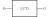
\includegraphics[width=0.3\linewidth]{D2_lut1}
                    \label{fig:D2_lut1}
                \end{figure}	
	
                Este elemento proporciona una versión de look-up table de un búfer o inversor. Estos elementos son los bloques de construcción básicos. El parámetro INIT le da a la LUT su valor lógico. De forma predeterminada, este valor es cero, lo que lleva la salida a cero independientemente de los valores de entrada (actuando como tierra).Sin embargo, en la mayoría de los casos hay que determinar un nuevo valor INIT para especificar la función lógica de la primitiva LUT. Existen al menos dos métodos mediante los cuales se puede determinar el valor LUT. El método de la tabla lógica y el método de ecuación. En la Tabla \ref{tab:lut1} se muestran las entradas y salidas y la forma de configurar INIT y en el Código \ref{cod:lut1} se muestra su implementación en VHDL.

                \begin{table}[htbp]
                    \centering
                    \caption{Tabla lógica de LUT1.}
                    \begin{tabular}{|cc|}
                        \hline
                        \multicolumn{1}{|c|}{\textbf{Inputs}} & \textbf{Outputs} \\ 
                        \multicolumn{1}{|c|}{\textbf{I0}} & \textbf{O} \\ 
                        \hline 
                        \multicolumn{1}{|c|}{0} & INIT[0] \\ \hline
                        \multicolumn{1}{|c|}{1} & INIT[1] \\ \hline
                        \multicolumn{2}{|c|}{INIT = Binary number assigned to the INIT attribute} \\ 
                        \hline
                    \end{tabular}
                    \label{tab:lut1}
                \end{table}	
	
                \vspace{0.4cm}
                \lstinputlisting[style = VHDL_TEXT, caption = Primitava de LUT1., label = cod:lut1]{codigos/vhdl_codes/primitivas/lut1.vhd}
                % \lstinputlisting[style = VHDL_TEXT]{codigos/vhdl_codes/primitivas/lut1.vhd}

            \subsubsection{OBUFDS: Differential Signaling Output Buffer}

                \begin{figure}[hbtp]
                    \caption{Esquemático de OBUFDS.}
                    \centering
                    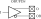
\includegraphics[width=0.3\linewidth]{D3_obufds}
                    \label{fig:D3_obufds}
                \end{figure}	

                Este elemento de diseño es un búfer de salida única que admite señalización diferencial de bajo voltaje. OBUFDS aísla el circuito interno y proporciona corriente de accionamiento para las señales que salen del chip. Su salida se representa como dos puertos distintos (O y OB), uno considerado el ``maestro'' y el otro el ``esclavo''. El maestro y el esclavo son fases opuestas de la misma señal lógica.  En la Tabla \ref{tab:obufds} se muestran las entradas y salidas y en el Código \ref{cod:obufds} se muestra su implementación en VHDL.
                
                \begin{table}[htbp]
                    \centering
                    \caption{Tabla lógica de OBUFDS.}
                    \begin{tabular}{|c|cc|}
                        \hline
                        \textbf{Inputs} & \multicolumn{2}{c|}{\textbf{Outputs}} \\ 
                        \textbf{I}      & \multicolumn{1}{c}{\textbf{O}}  & \textbf{OB} \\ 
                        \hline
                        0      & \multicolumn{1}{c|}{0}  & 1  \\ \hline
                        1      & \multicolumn{1}{c|}{1}  & 0  \\ \hline
                    \end{tabular}
                    \label{tab:obufds}
                \end{table}

                \vspace{0.4cm}
                \lstinputlisting[style = VHDL_TEXT, caption = Primitava de OBUFDS., label = cod:obufds]{codigos/vhdl_codes/primitivas/obufds.vhd}
                % \lstinputlisting[style = VHDL_TEXT]{codigos/vhdl_codes/primitivas/obufds.vhd}

                La libreria del proyecto HECTOR \cite{Laban2016} hace uso de estas libreria para describir el ERO-TRNG y parametríza el número de buffers para fácil modificación de los retardos.

